

\subsection{P0 derived network to stratify MIBC} \label{s:p0}

 
The Jack Birch's Unit holds a large dataset of bladder tissue samples both cancerous and non-cancerous. There are three different types of 'normal'  (or healthy or non-cancerous) bladder samples: P0 (23), Abs/Ca-differentiated (49) and undifferentiated (15). The P0 are in-situ tissues taken from healthy individual unaltered in the lab, the ABS/Ca differentiated are in-vitro which have been differentiated by the ABS/Ca protocol and lastly the undifferentiated are in-vitro samples which tissues are yet not specialised. From the previous classifications \citet{Robertson2017-mg, Kamoun2020-tj} it is known that there are 2 major subgroups Luminal Papillary (Lum) and Basal Squamous (Ba). The former is known to share aspects with the differentiated tissue while the latter with the undifferentiated. 

In this section only the P0 dataset is used to construct a healthy network representing the co-expressed genes network in an unaltered bladder tissue. The network is built based on the pipeline described in Figure \ref{fig:N_I:network_pipeline} where instead of the tumour's gene expression the P0 RNAseq data is used, but the mutation burden for the modifiers is still used. This means that the Module Connectivity (ModCon) selects the genes which are most representative of the communities in the healthy network. These selected genes are used to compute the Module Evaluation Value score using the gene expression from TCGA. Therefore, this approach can be thought as a method to select the genes most representative for the P0 samples and how their expression in the tumours dataset inform the MIBC subtyping. 

It is worth noting that there are only 23 P0 samples and this may not offer enough statistical power to find communities with specific biological functions. In addition, the Basal may be under-represented by the lack of undifferentiated tissue samples. Nevertheless, using unprocessed tissue samples may unravel new biology.

The minimum degree for TF was pseudo-empirical chosen when several networks were generated with TF 10-100 (25 steps) and visualised in Gephi. It was then observed that networks with higher number of edges were very nested and harder to analysed with lower scores. It was also (wrongly) assumed that Leiden algorithm would not be heavily influenced by allowing TF (~325 of 4000 genes) more links. To put things in perspective, the Spearman correlation matrix us 4000x4000 and each gene has 3999 correlations. Thus keeping 100 genes for each TF does not seem a lot. However, the experiments in this section and the work in Section \ref{}\footnote{Selective edge pruning experiment} will show that allowing such a large number of TF has a big impact on the number of communities.

In PGCNA \citet{Care2019-ij} the authors select in each community the top 25 genes with the highest ModCon score. This was the initial value used in the P0 experiments too but then it was noticed that many genes are missed, where communities in the healthy were not expressed in tumours. Thus, it was increased to 100.

Therefore, in this section the top 4K most-relative varied genes (median/std) from P0 are used to construct the network, the same weight modifiers (Reward and Penalised see Figure \ref{fig:N_I:modifiers}) are employed and 50 edges for the Transcription Factor. For the standard genes 3 edges are kept while for Transcription Factors (TFs) 50. The top 100 genes are selected with ModCon and for MEVs the top 4K most varied genes are used.

\subsubsection{Describing the Network}


\begin{figure}[!htb]    
    \centering
    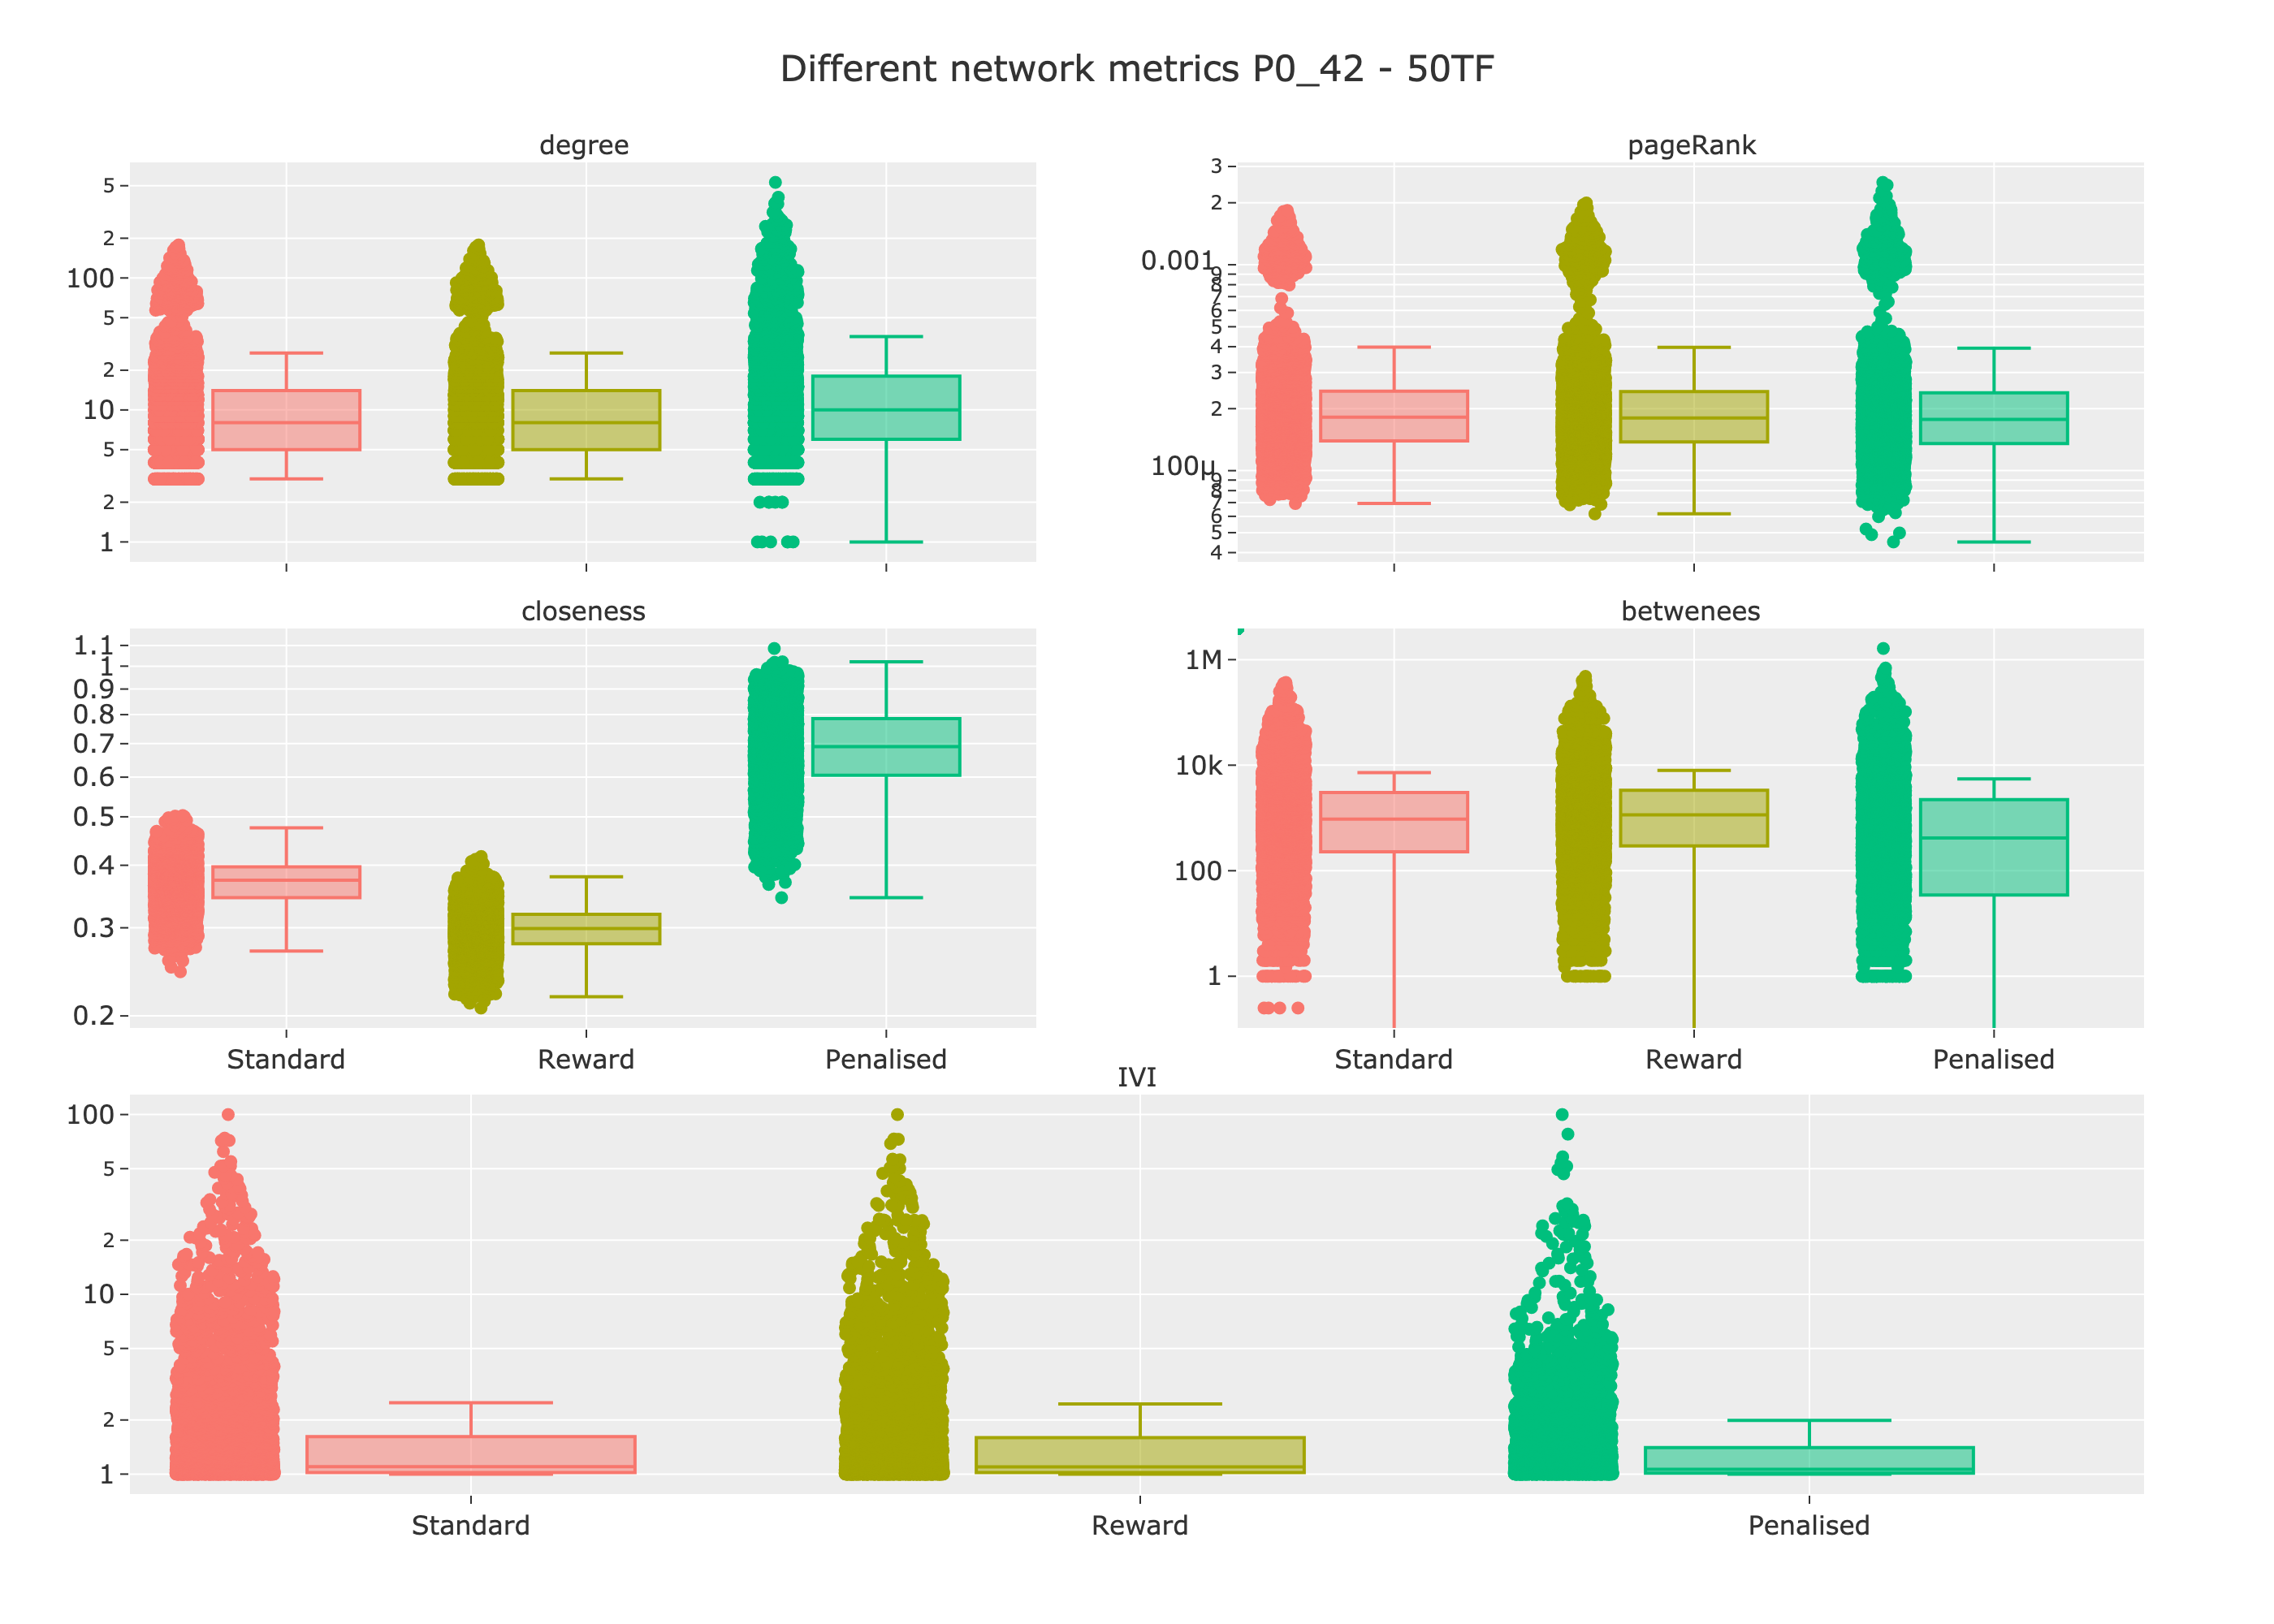
\includegraphics[width=1.0\textwidth,height=0.7\textheight,keepaspectratio]{Sections/Network_I/Resources/P0/P0_NetworkMetricsComp_50TF_2.png}
    \caption{Network metrics for the P0 networks formed from 4K genes, 3 connections per standard gene and 50 for TFs with the different weight modifiers; standard (blue), reward (red) and penalised (green). The y-axis represent the log10 of the metric. }
    \label{fig:N_I:net_metrics_p0}
\end{figure}

In the previous section \ref{s:N_I:tum_describe} five different network metrics were chosen to describe the networks generated: degree, PageRank, closeness, betweeness and IVI. These give an overview of the network properties, how well are the nodes connected, shortest path between them and their overall importance (IVI). In Figure \ref{fig:N_I:net_metrics_p0} the degree and PageRank plots for Standard and Reward network have a cone-like set of points, denoting a subgroup of genes with a high number of edges. This is further enforced by the scale of the Y-axes; compared to the tumour experiments where the nodes degree where $<100$. Interestingly, PageRank values are at the similar scale with the ones from the tumour experiments (Figure \ref{fig:N_I:net_metrics_tum}). From the Closeness plot it can be seen that the Reward and Standard have lower values compared to Penalised denoting that less central nodes in the networks. For the Integrated Value Of Influence (IVI) the Standard and Reward have a larger spread compared to Penalised. 

Overall, the network metrics shows that the Penalised network is different from the other two networks suggesting that reducing the weights to values close to 0 for highly mutated genes has a higher impact on the network than doubling their values.

\subsubsection{Choosing Clustering model} \label{s:p0:clustering_analysis}

% Explain what and why are the clustering methods we used
To find the appropriate clustering model and the number of clusters we adapt the previous work done in Chapter \ref{}\footnote{Subtyping chapter} where we used Principal Component Analysis (PCA) and K-means to stratify MIBC based on gene expression. Based on three different clustering method (Silhouette with cosine distance, Calinski Habrasz and Davies Bouldin\footnote{For a refresher on the clustering metrics see Section \ref{}}) we selected following clustering models \footnote{I have explored other clustering methods such as DBSCAN, MeanShit, Affinity Propagation, OPTICS, HDBSCAN and Fuzzy K-means. All based on Scikit-learn \cite{Scikit-learn_undated-ax}} the K-means, Agglomerative Clustering with Average linkage (Agg\_Avg), Birch, Ward, Gaussian Mixture Model and Spectral Clustering. 

\begin{figure}[!htb]
    \centering
    \begin{subfigure}[b]{0.49\textwidth}
        \centering
        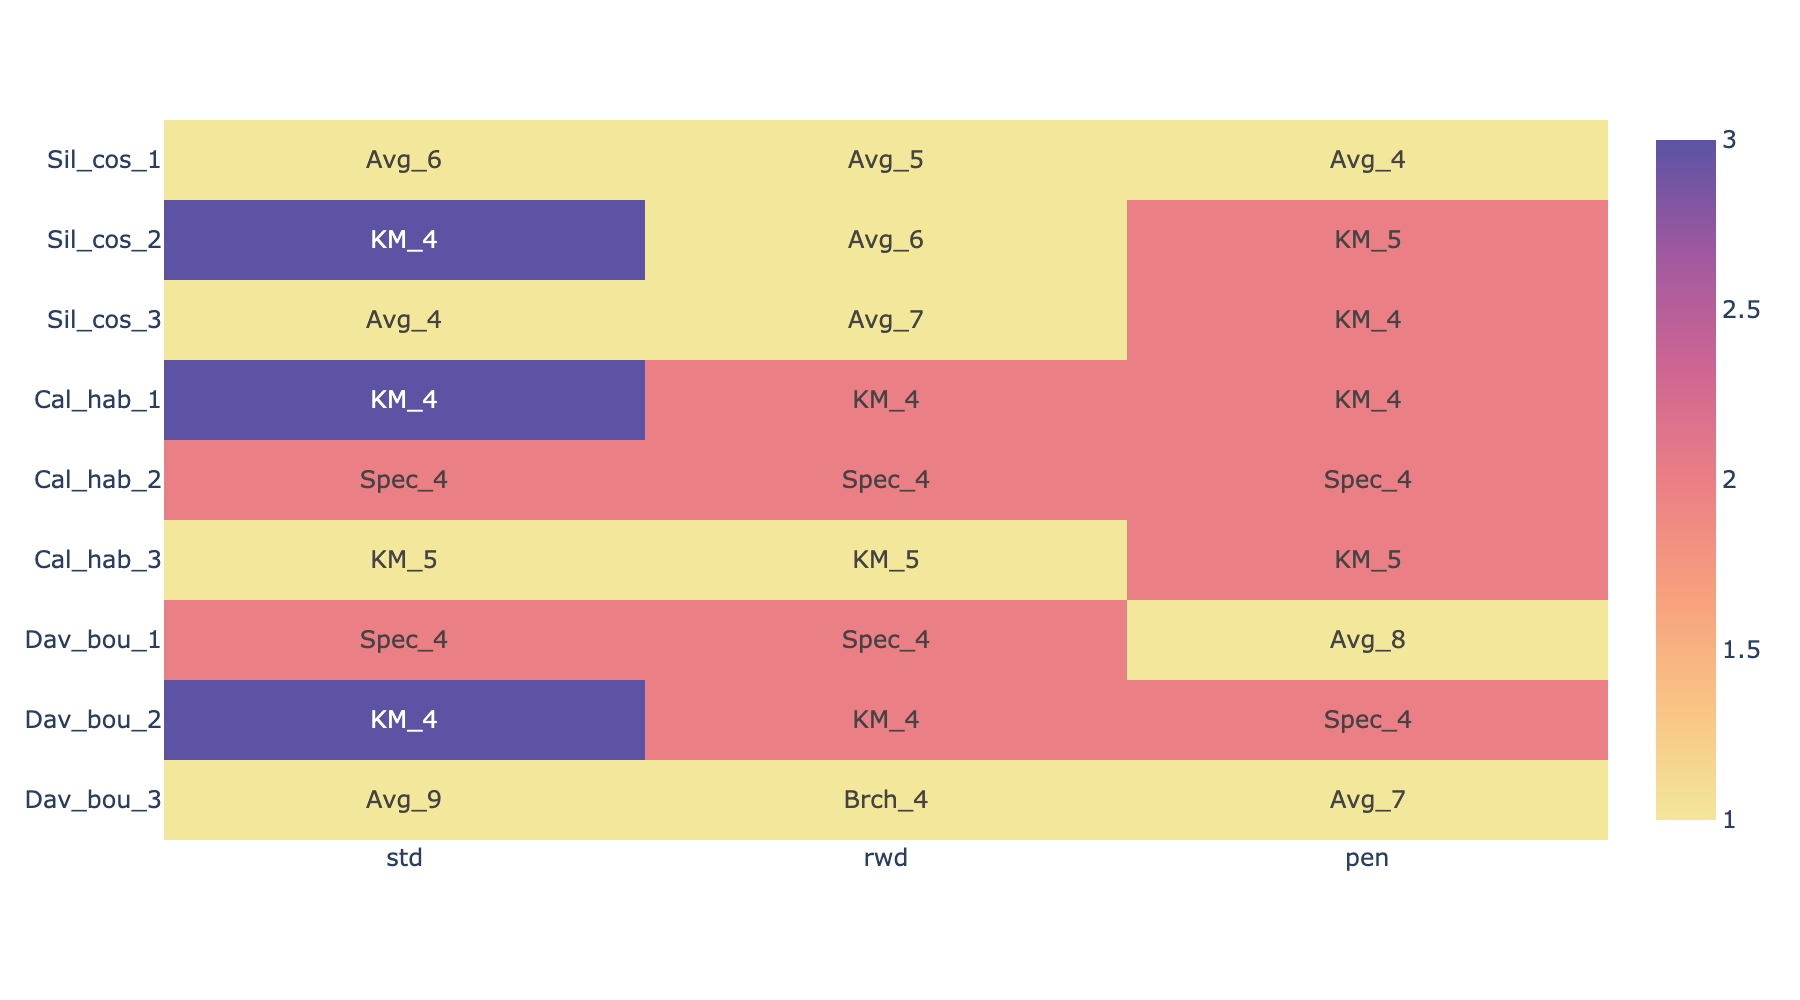
\includegraphics[width=\textwidth,keepaspectratio]{Sections/Network_I/Resources/P0/top3_cs_gen_p0_tum4K.png}    
        \caption{Cluster model and size}
    \end{subfigure}
    \hfill
    \begin{subfigure}[b]{0.49\textwidth}
        \centering
        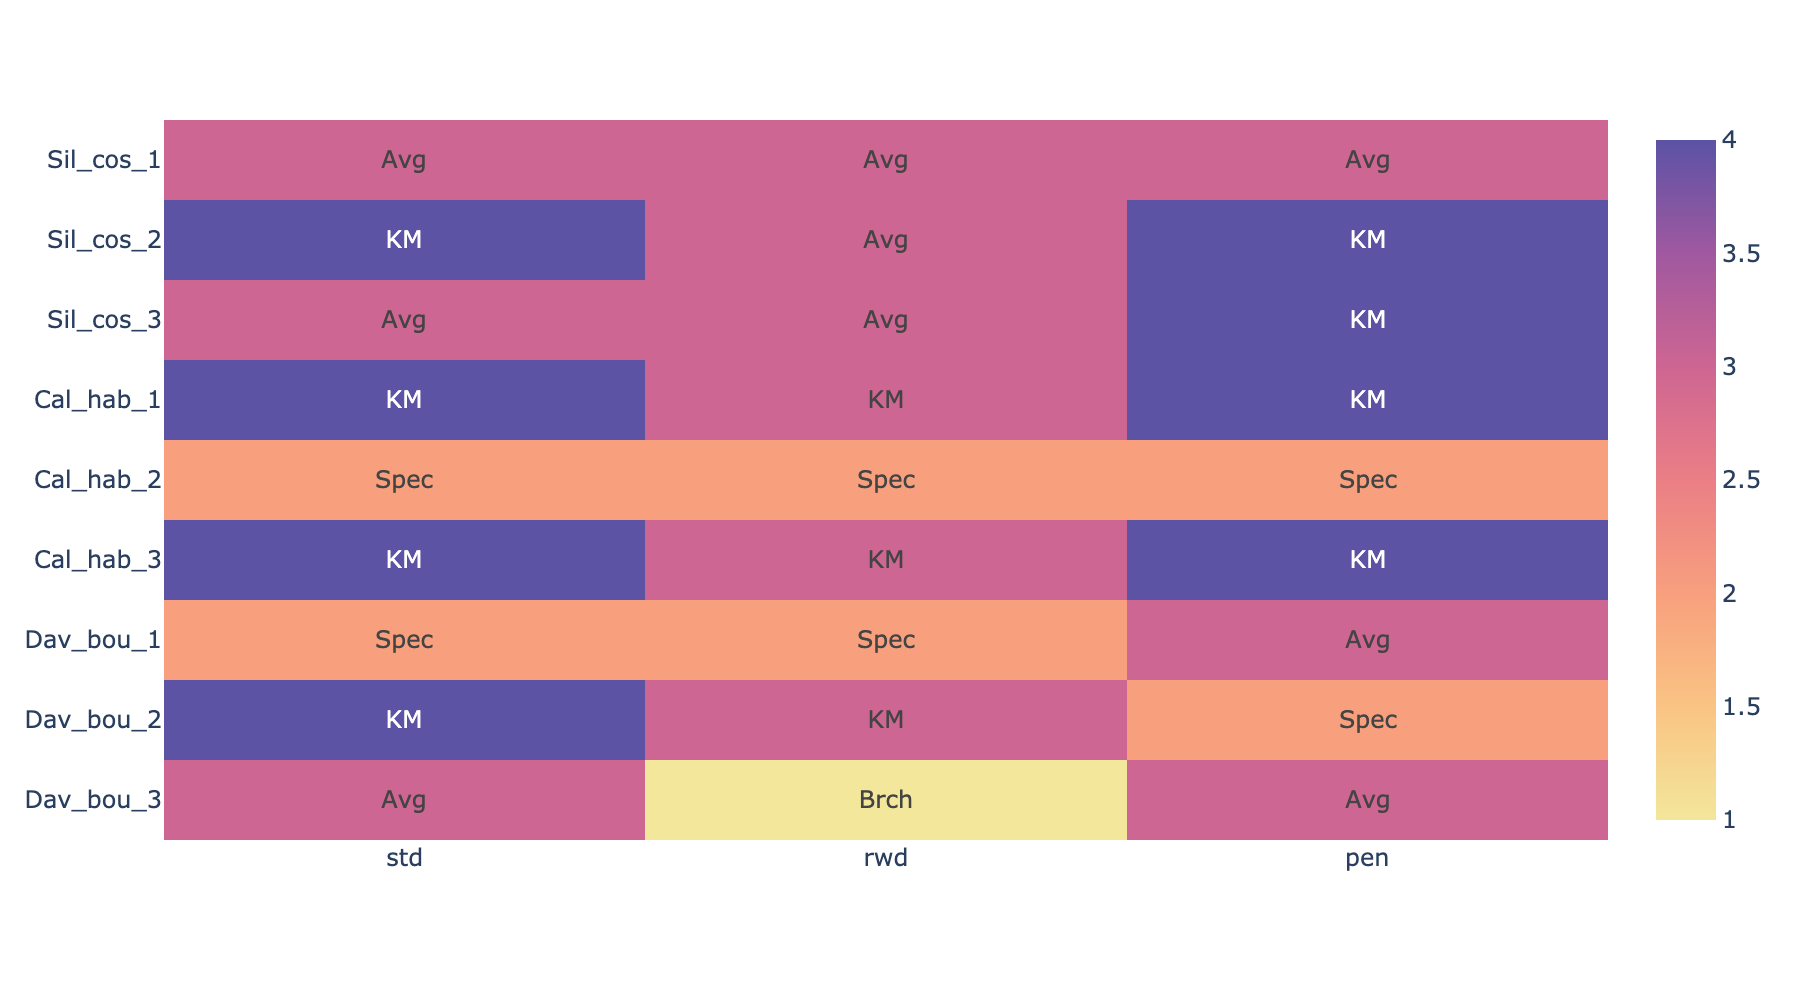
\includegraphics[width=\textwidth,keepaspectratio]{Sections/Network_I/Resources/P0/top3_cs_model_p0_tum4K.png}
        \caption{Cluster model}
    \end{subfigure} %
    \hfill
    \begin{subfigure}[b]{0.49\textwidth}
        \centering
        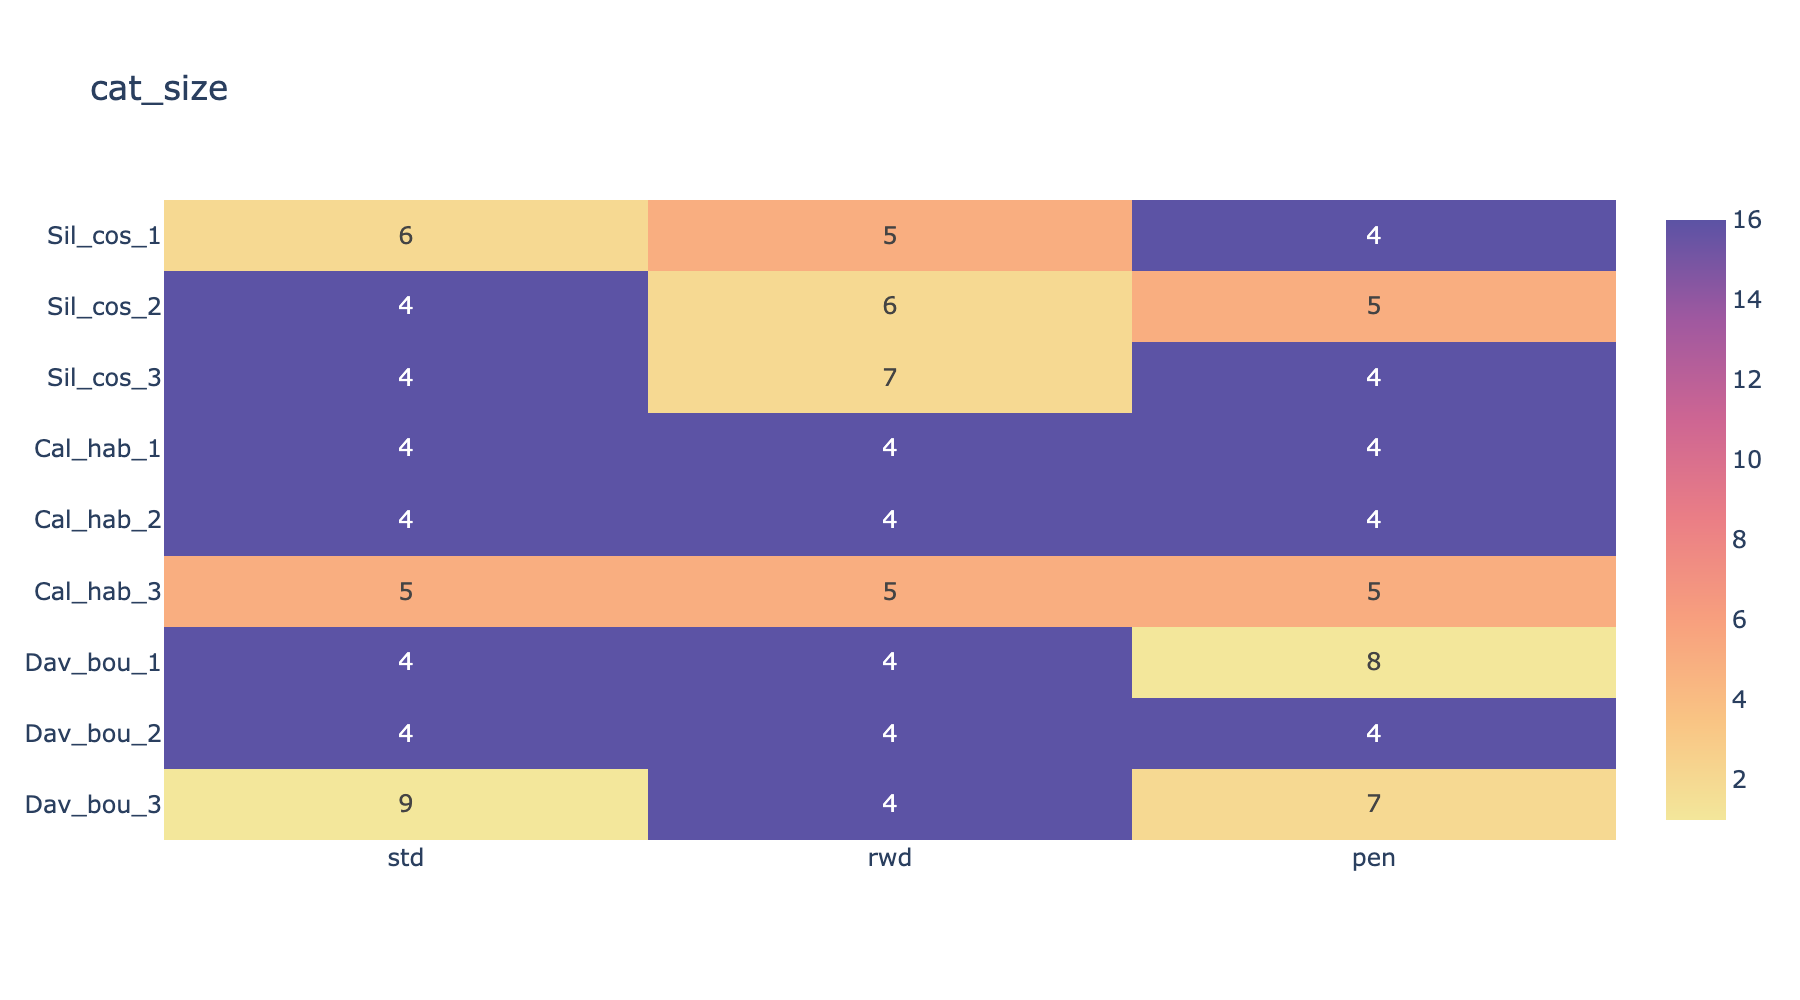
\includegraphics[width=\textwidth,keepaspectratio]{Sections/Network_I/Resources/P0/top3_cs_size_p0_tum4K.png}
        \caption{Cluster size}
    \end{subfigure}
     \hfill
    \begin{subfigure}[b]{0.49\textwidth}
        \centering
        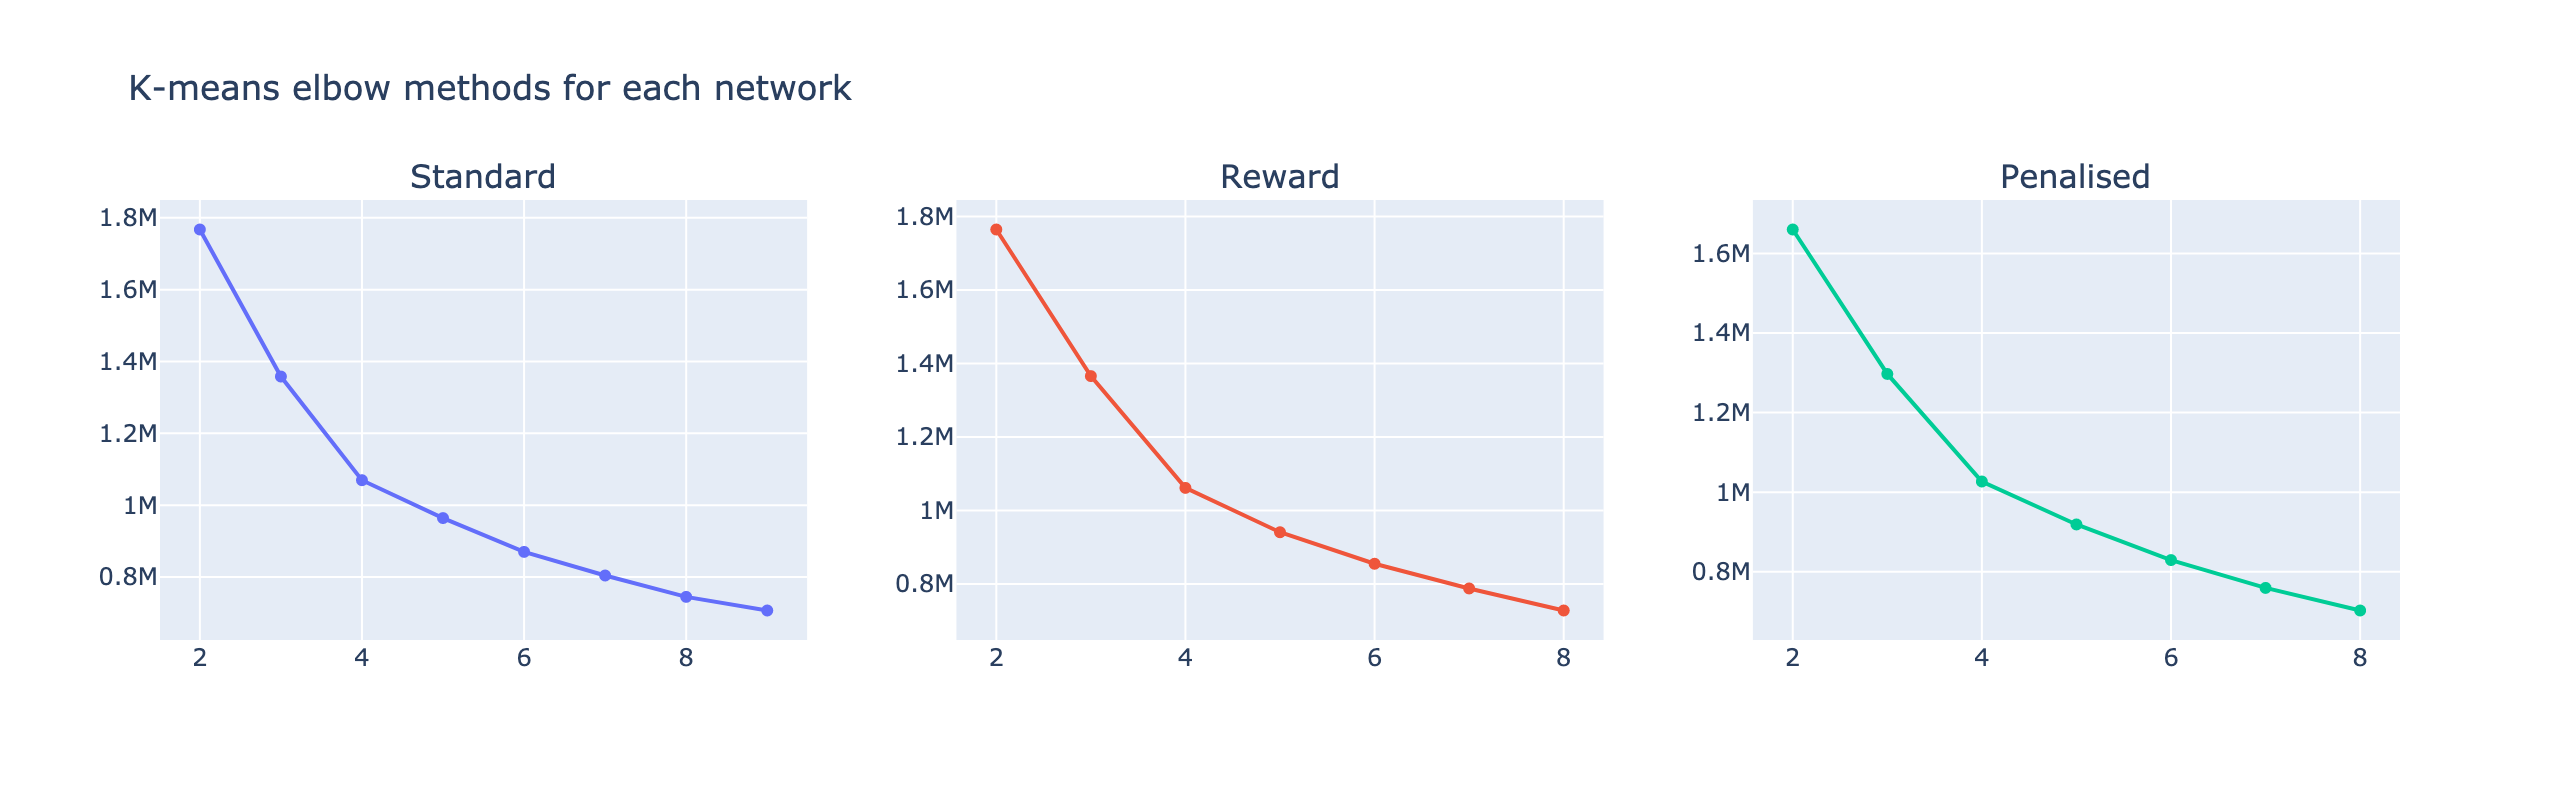
\includegraphics[width=\textwidth, keepaspectratio]{Sections/Network_I/Resources/P0/p0_elbowMethod_4K.png}
        \label{fig:N_I:p0_elbow_method}
        \caption{Elbow method}
    \end{subfigure}
    \caption{Clustering models for each network type with the top three clustering scores. Colouring scale corresponds to the encounter frequency \textbf{per network type}; i.e. the count restarts for every network. A) looks at the overall most common clustering model configuration. B) at the most common clustering model C) the most likely cluster size.}
    \label{fig:N_I:p0_top_3_metrics}
\end{figure}


% Introduce the results and motivate the reason of why we don't include K=2,3
In this section we apply the above-mentioned clustering methods to the MEV scores derived from the three networks (Standard, Reward and Penalised) with K ranging from 3-9 and we used the same clustering metrics to assess the performance. Importantly, the models with 2 clusters or 3 are not taken in account as the metrics tend to give higher score for models with 2,3 clusters. In Figure \ref{fig:N_I:p0_choosing_cs} the clustering metrics are displayed, were the number of 'x' marks the highest score after cluster size 2 and 3.This can be seen in our results as well were usually the clustering models perform worst with the increase of K. 

\begin{figure}[!htb]
    \thispagestyle{plain}
    \centering
    \begin{subfigure}{1.0\linewidth}
        \centering
        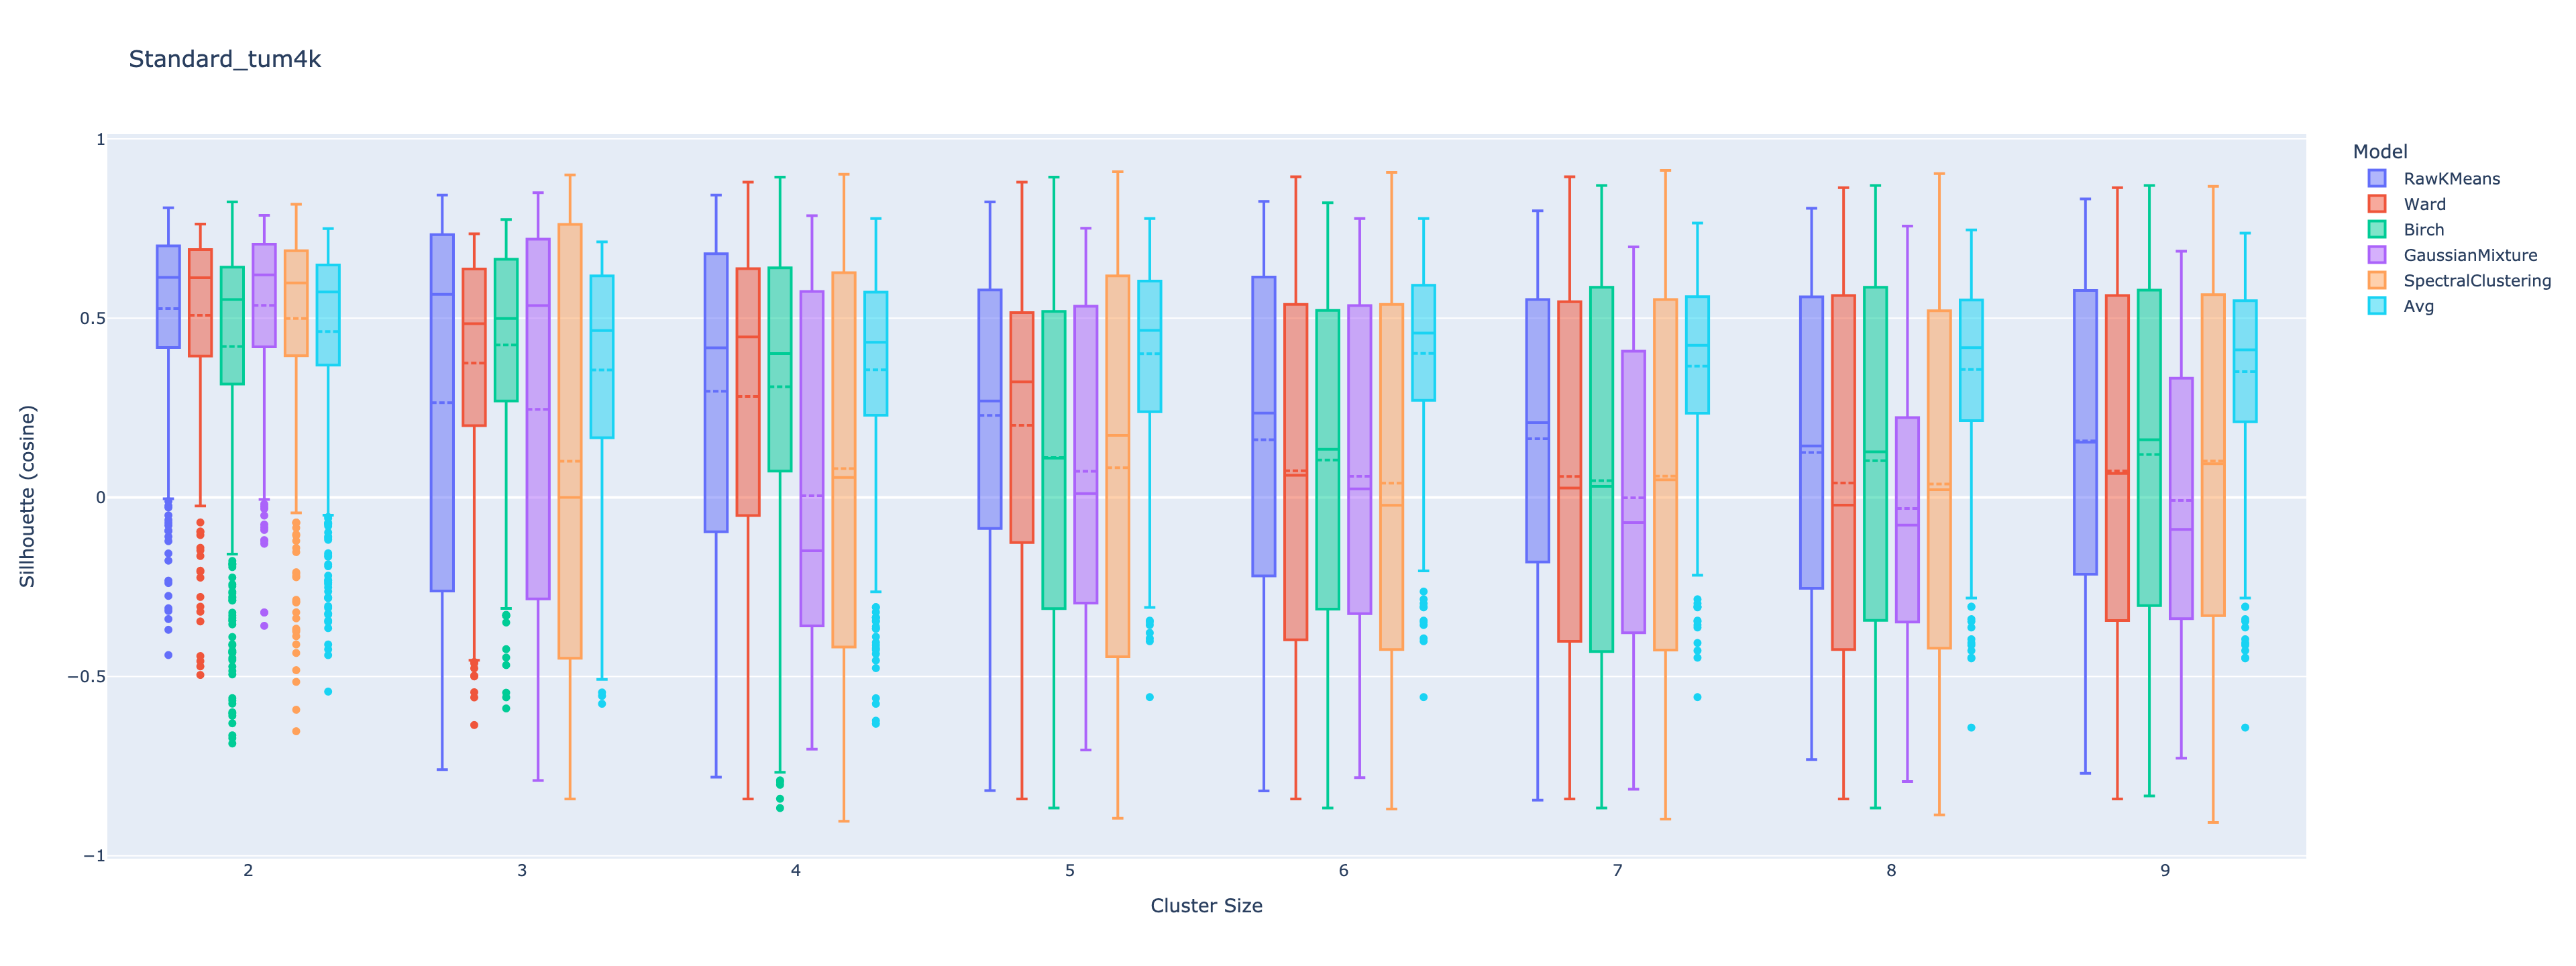
\includegraphics[width=1.0\textwidth,height=0.17\textheight]{Sections/Network_I/Resources/P0/Standard_tum4k_sill_spread.png}
        \caption{Standard network}
    \end{subfigure} %

    \begin{subfigure}{1.0\linewidth}
        \centering
        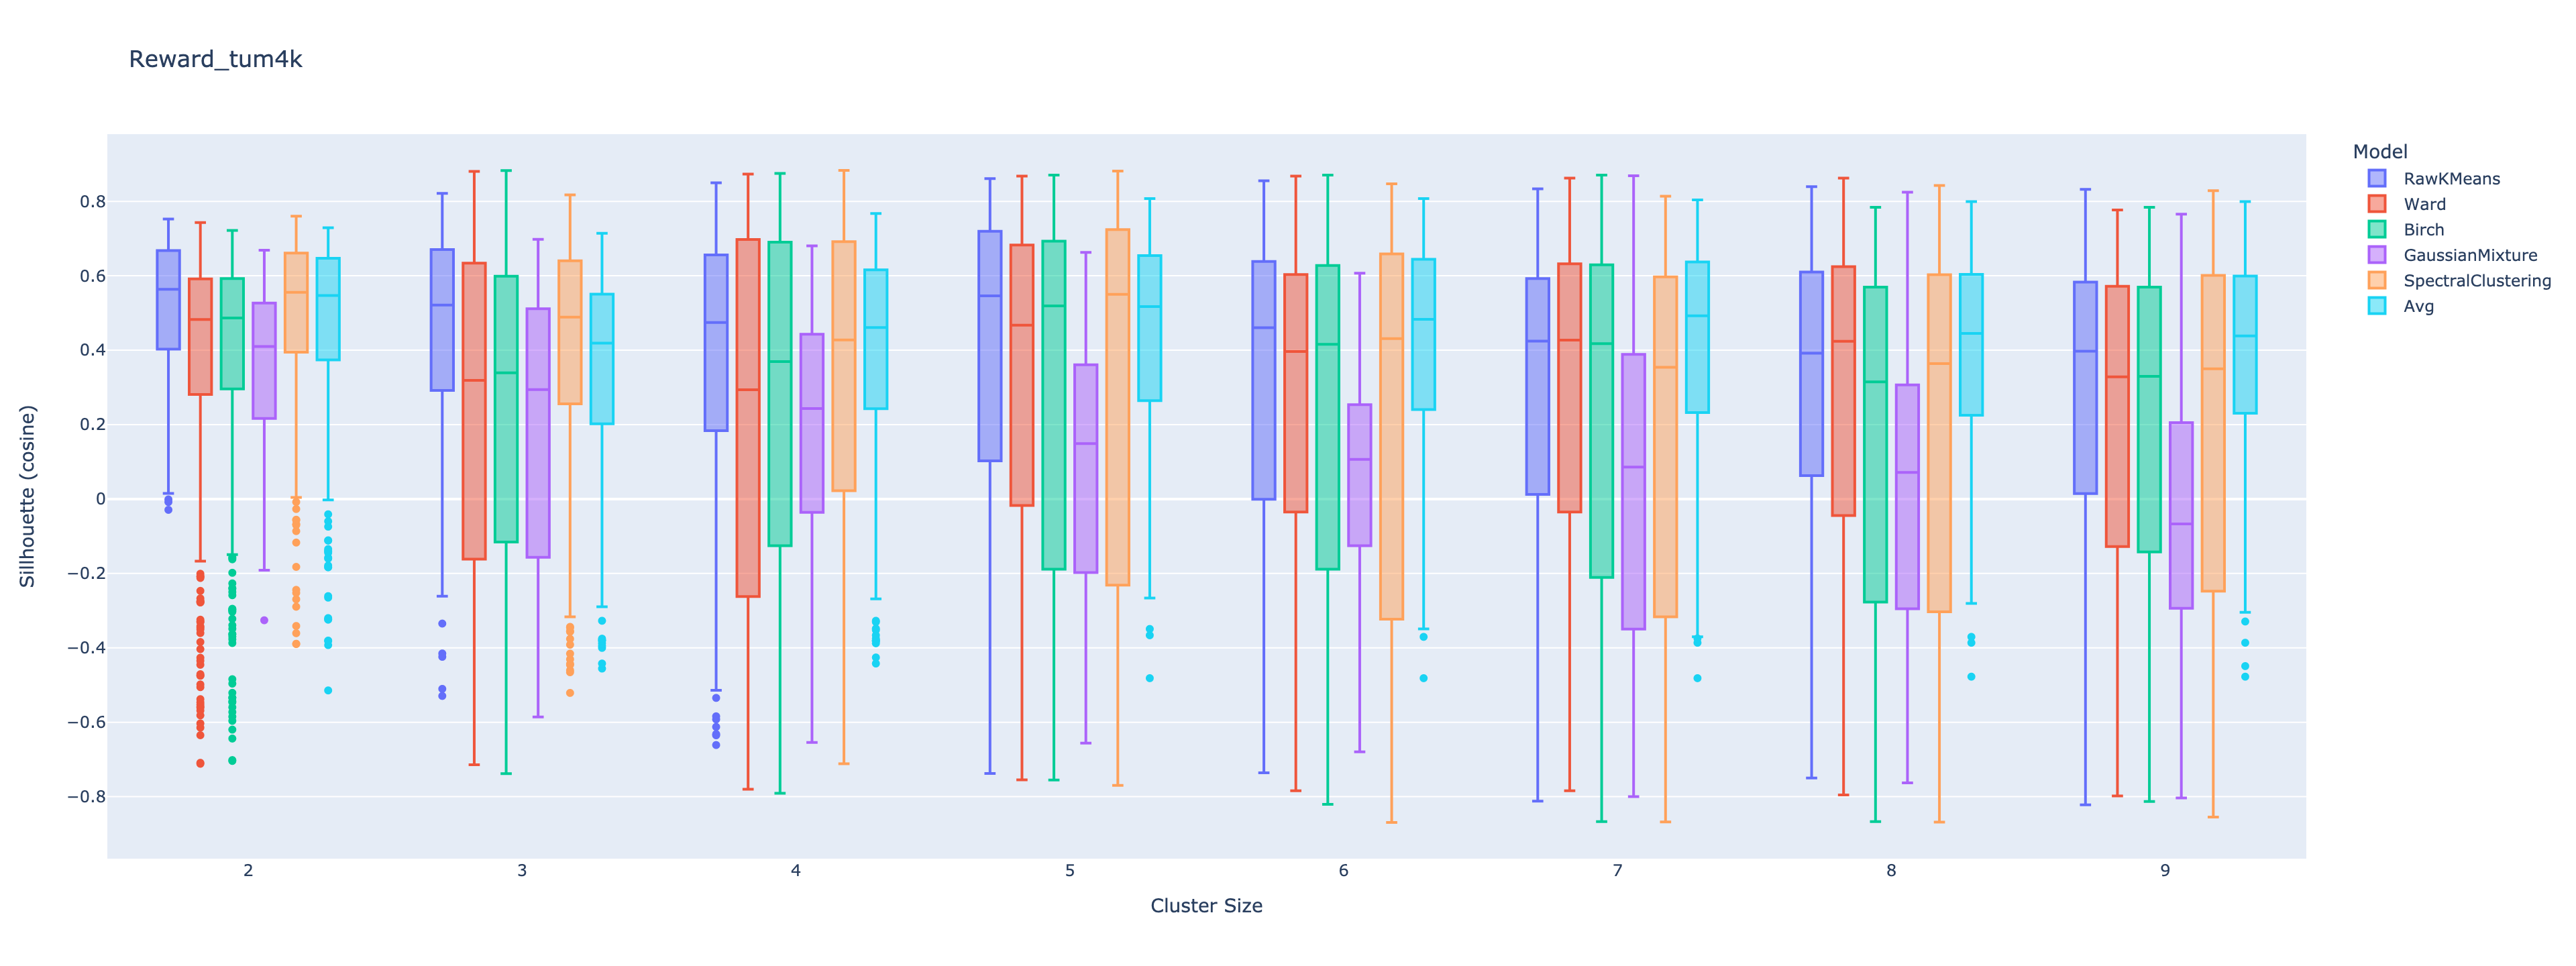
\includegraphics[width=1.0\textwidth,height=0.17\textheight]{Sections/Network_I/Resources/P0/Reward_tum4k_sill_spread.png}
        \caption{Reward network}
    \end{subfigure}
    
    \begin{subfigure}{1.0\linewidth}
        \centering
        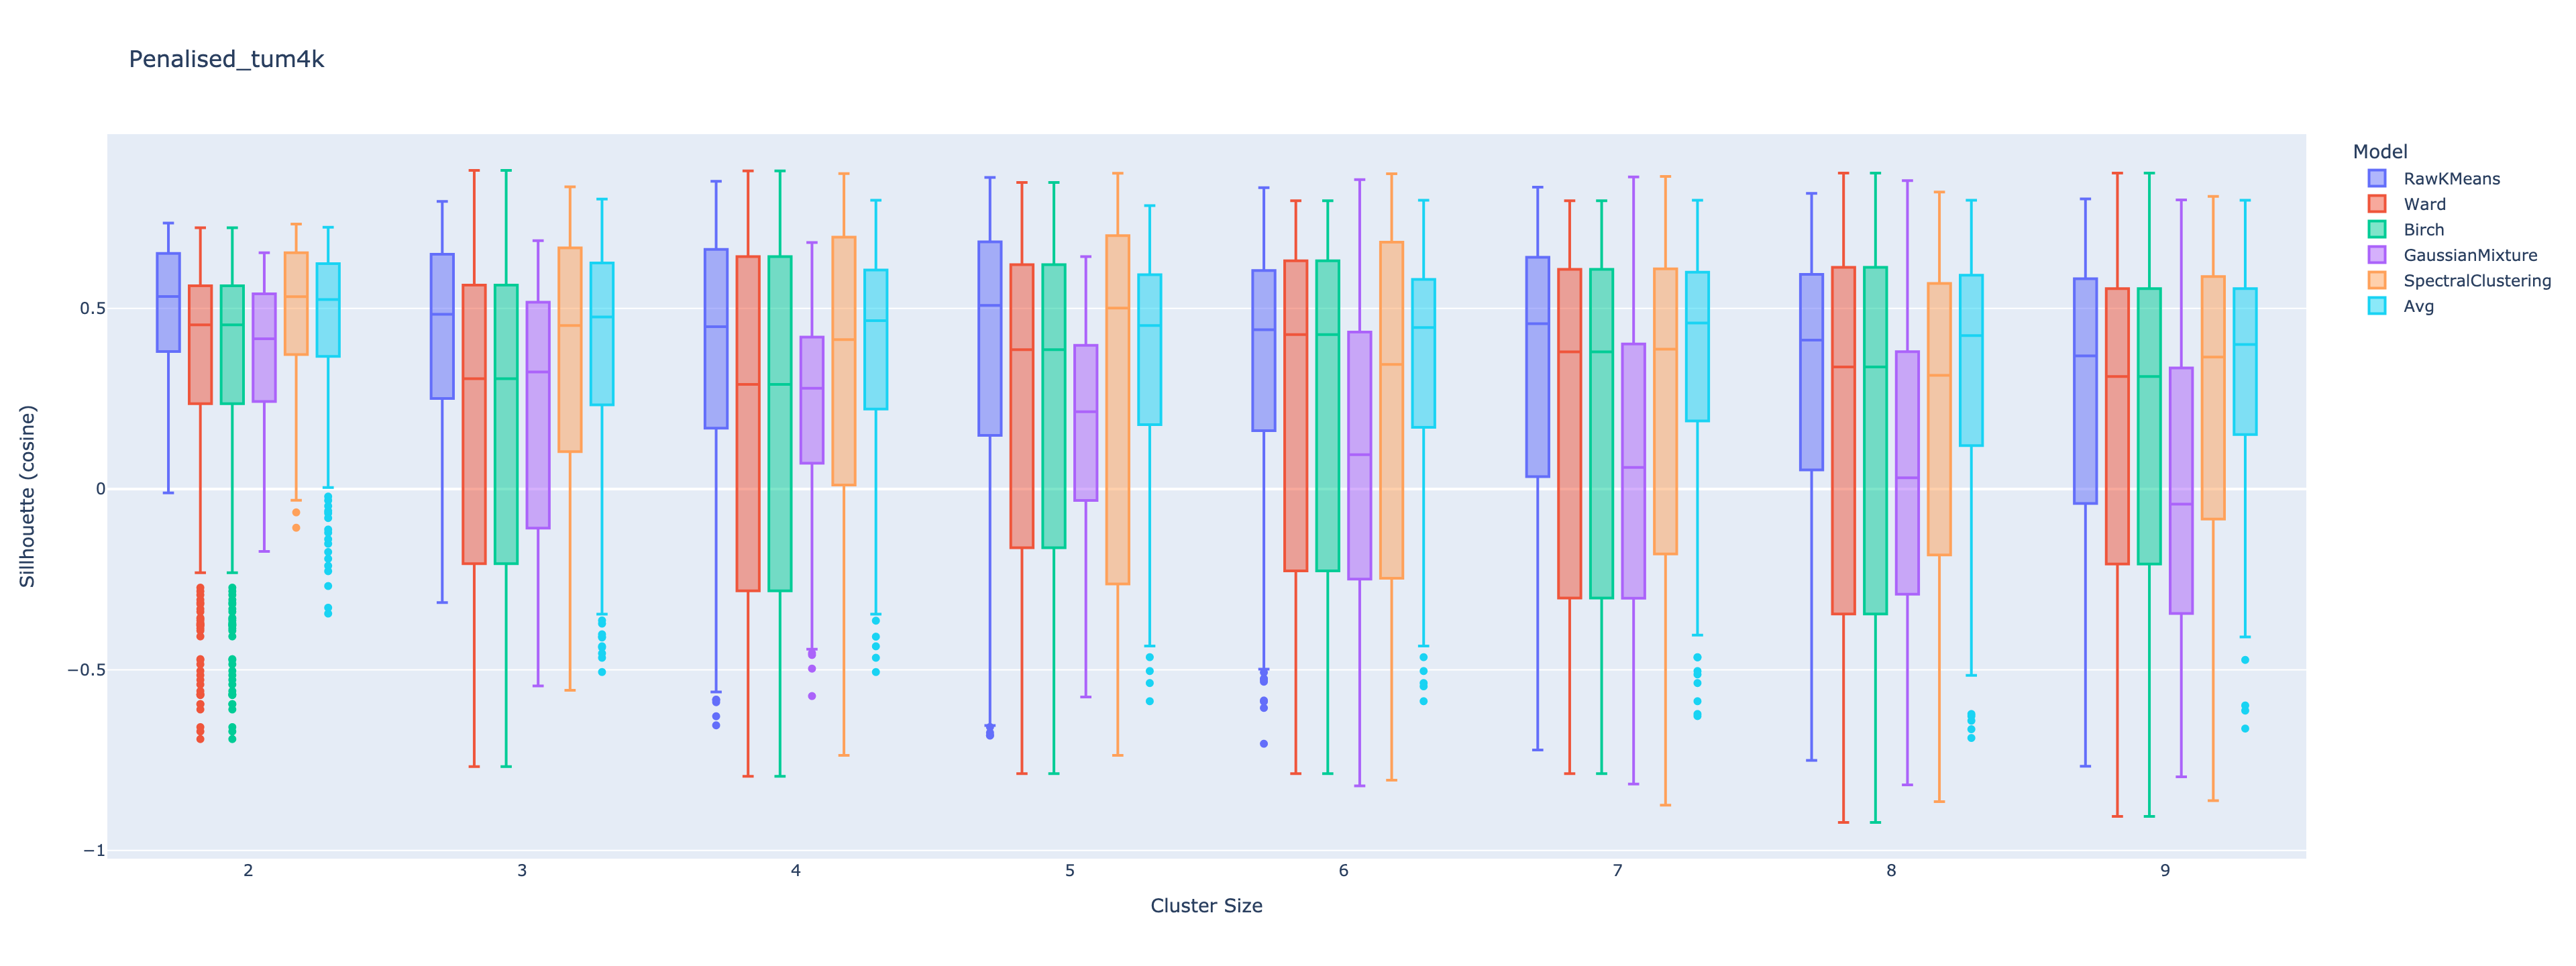
\includegraphics[width=1.0\textwidth,height=0.17\textheight]{Sections/Network_I/Resources/P0/Penalised_tum4k_sill_spread.png}      
        \caption{Penalised network}
    \end{subfigure}
    \caption{Cosine Silhouette score spread across samples over different clustering models with various K.}
    \label{fig:N_I:p0_sillhouette_spread}
\end{figure}

\begin{figure}[!htb]
    \hfill
    \begin{subfigure}{1.0\linewidth}
        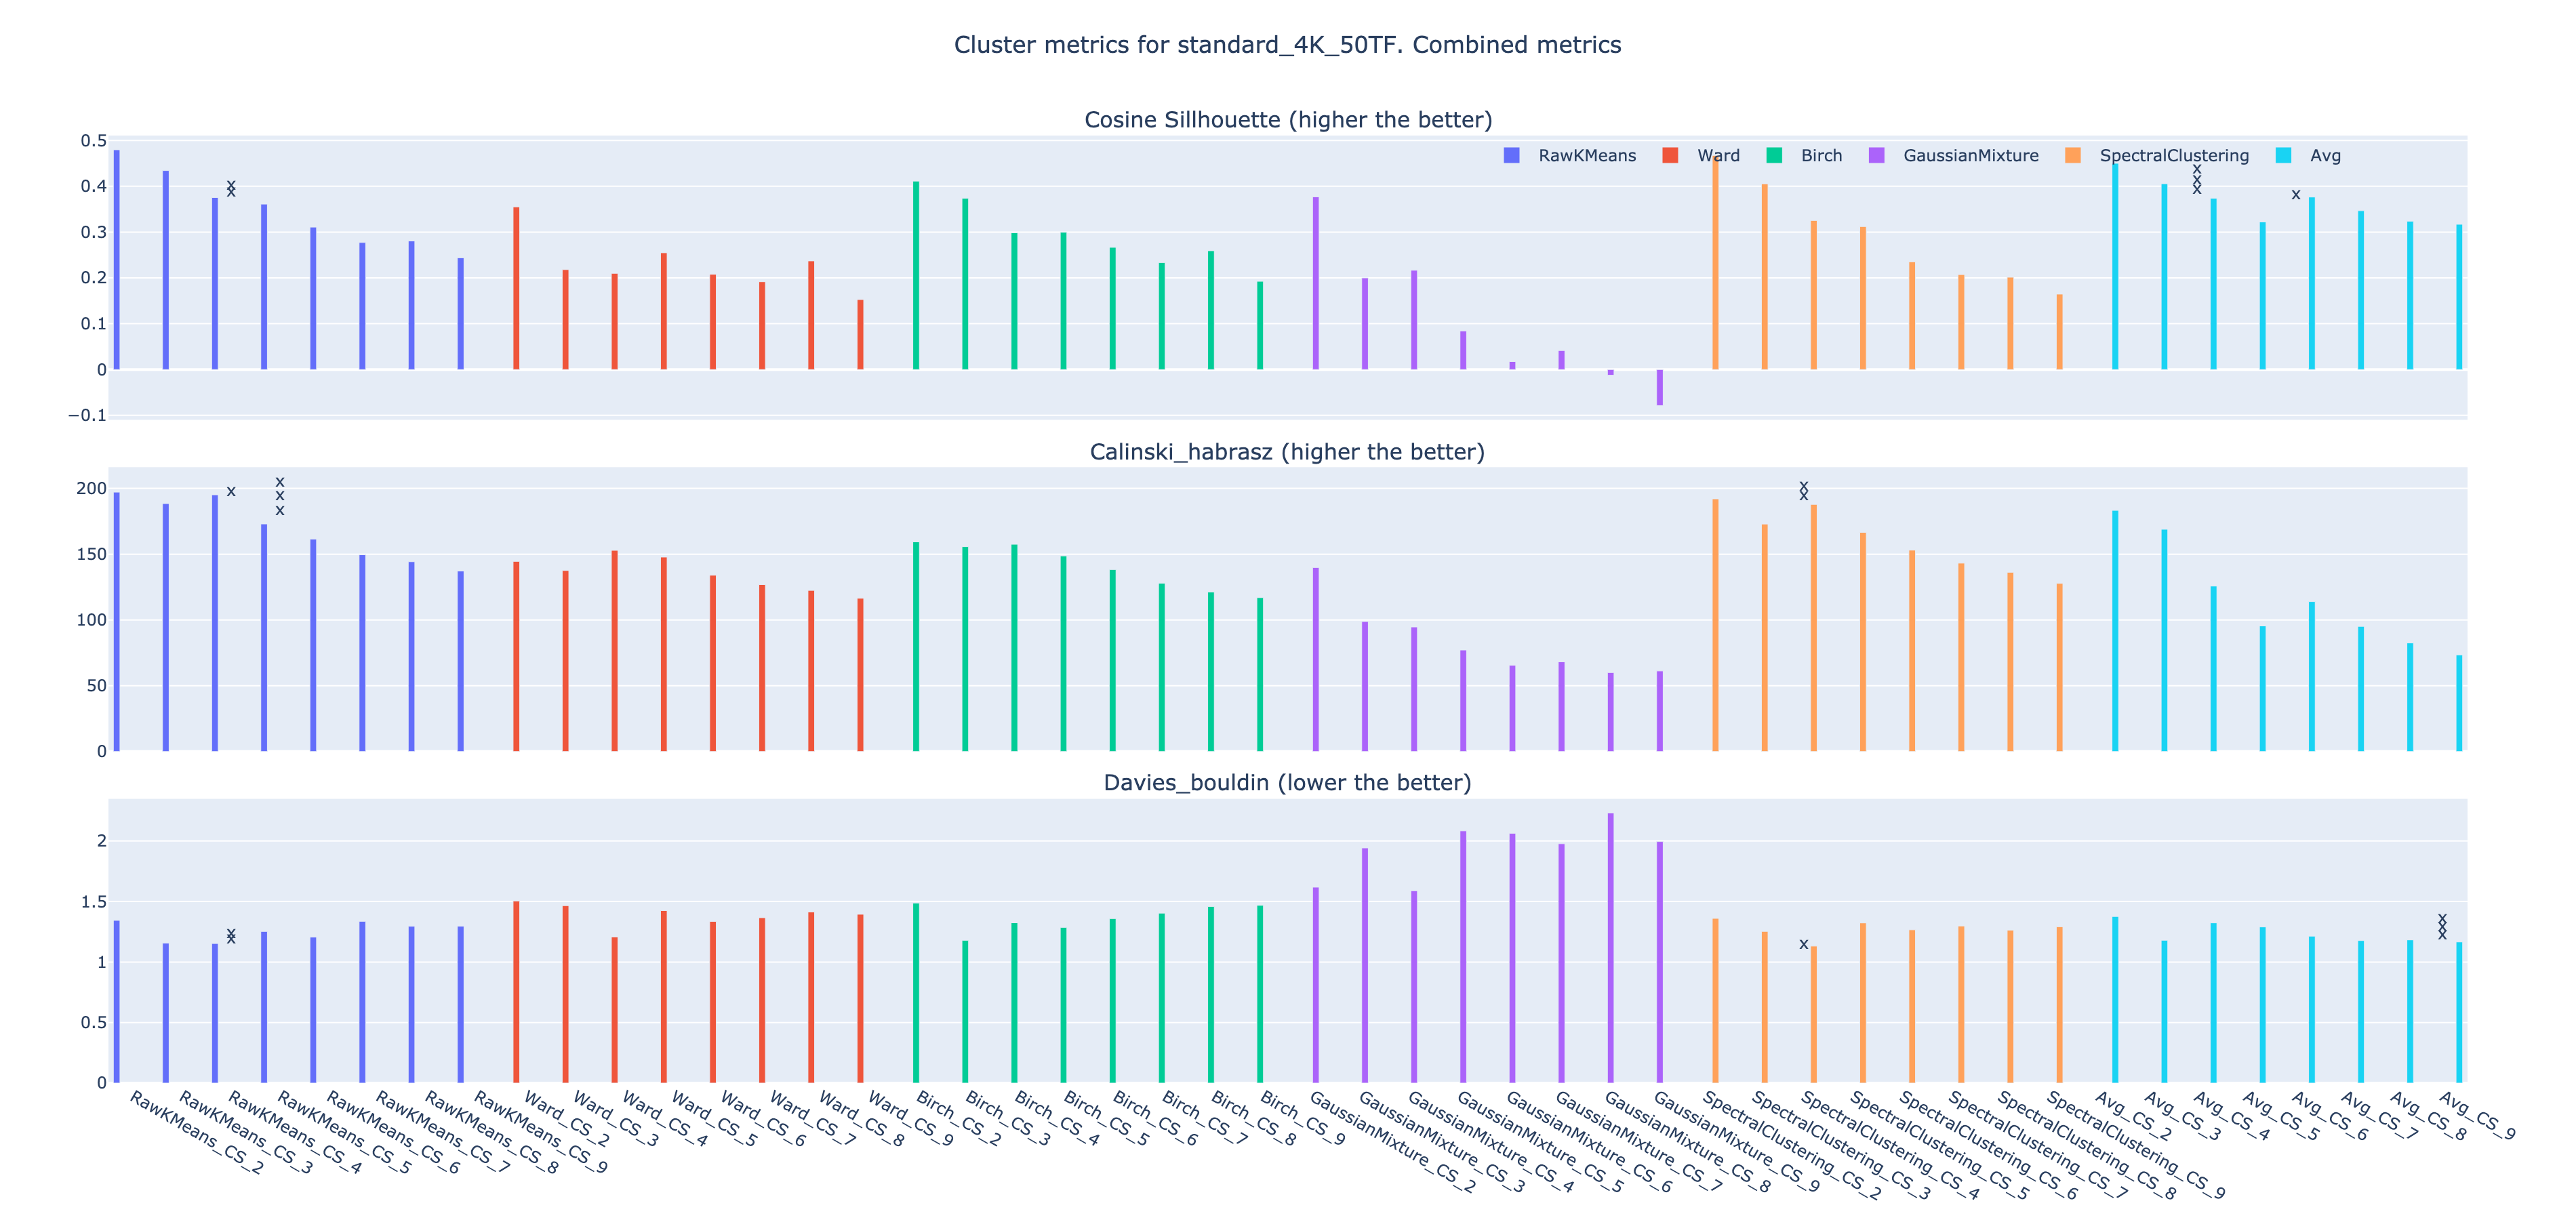
\includegraphics[width=1.0\textwidth,height=0.25\textheight]{Sections/Network_I/Resources/P0/CA_metrics_Std_2_tum_4k.png}
        \caption{Standard network}
    \end{subfigure} %
    \hfill
    \begin{subfigure}{0.49\linewidth}
        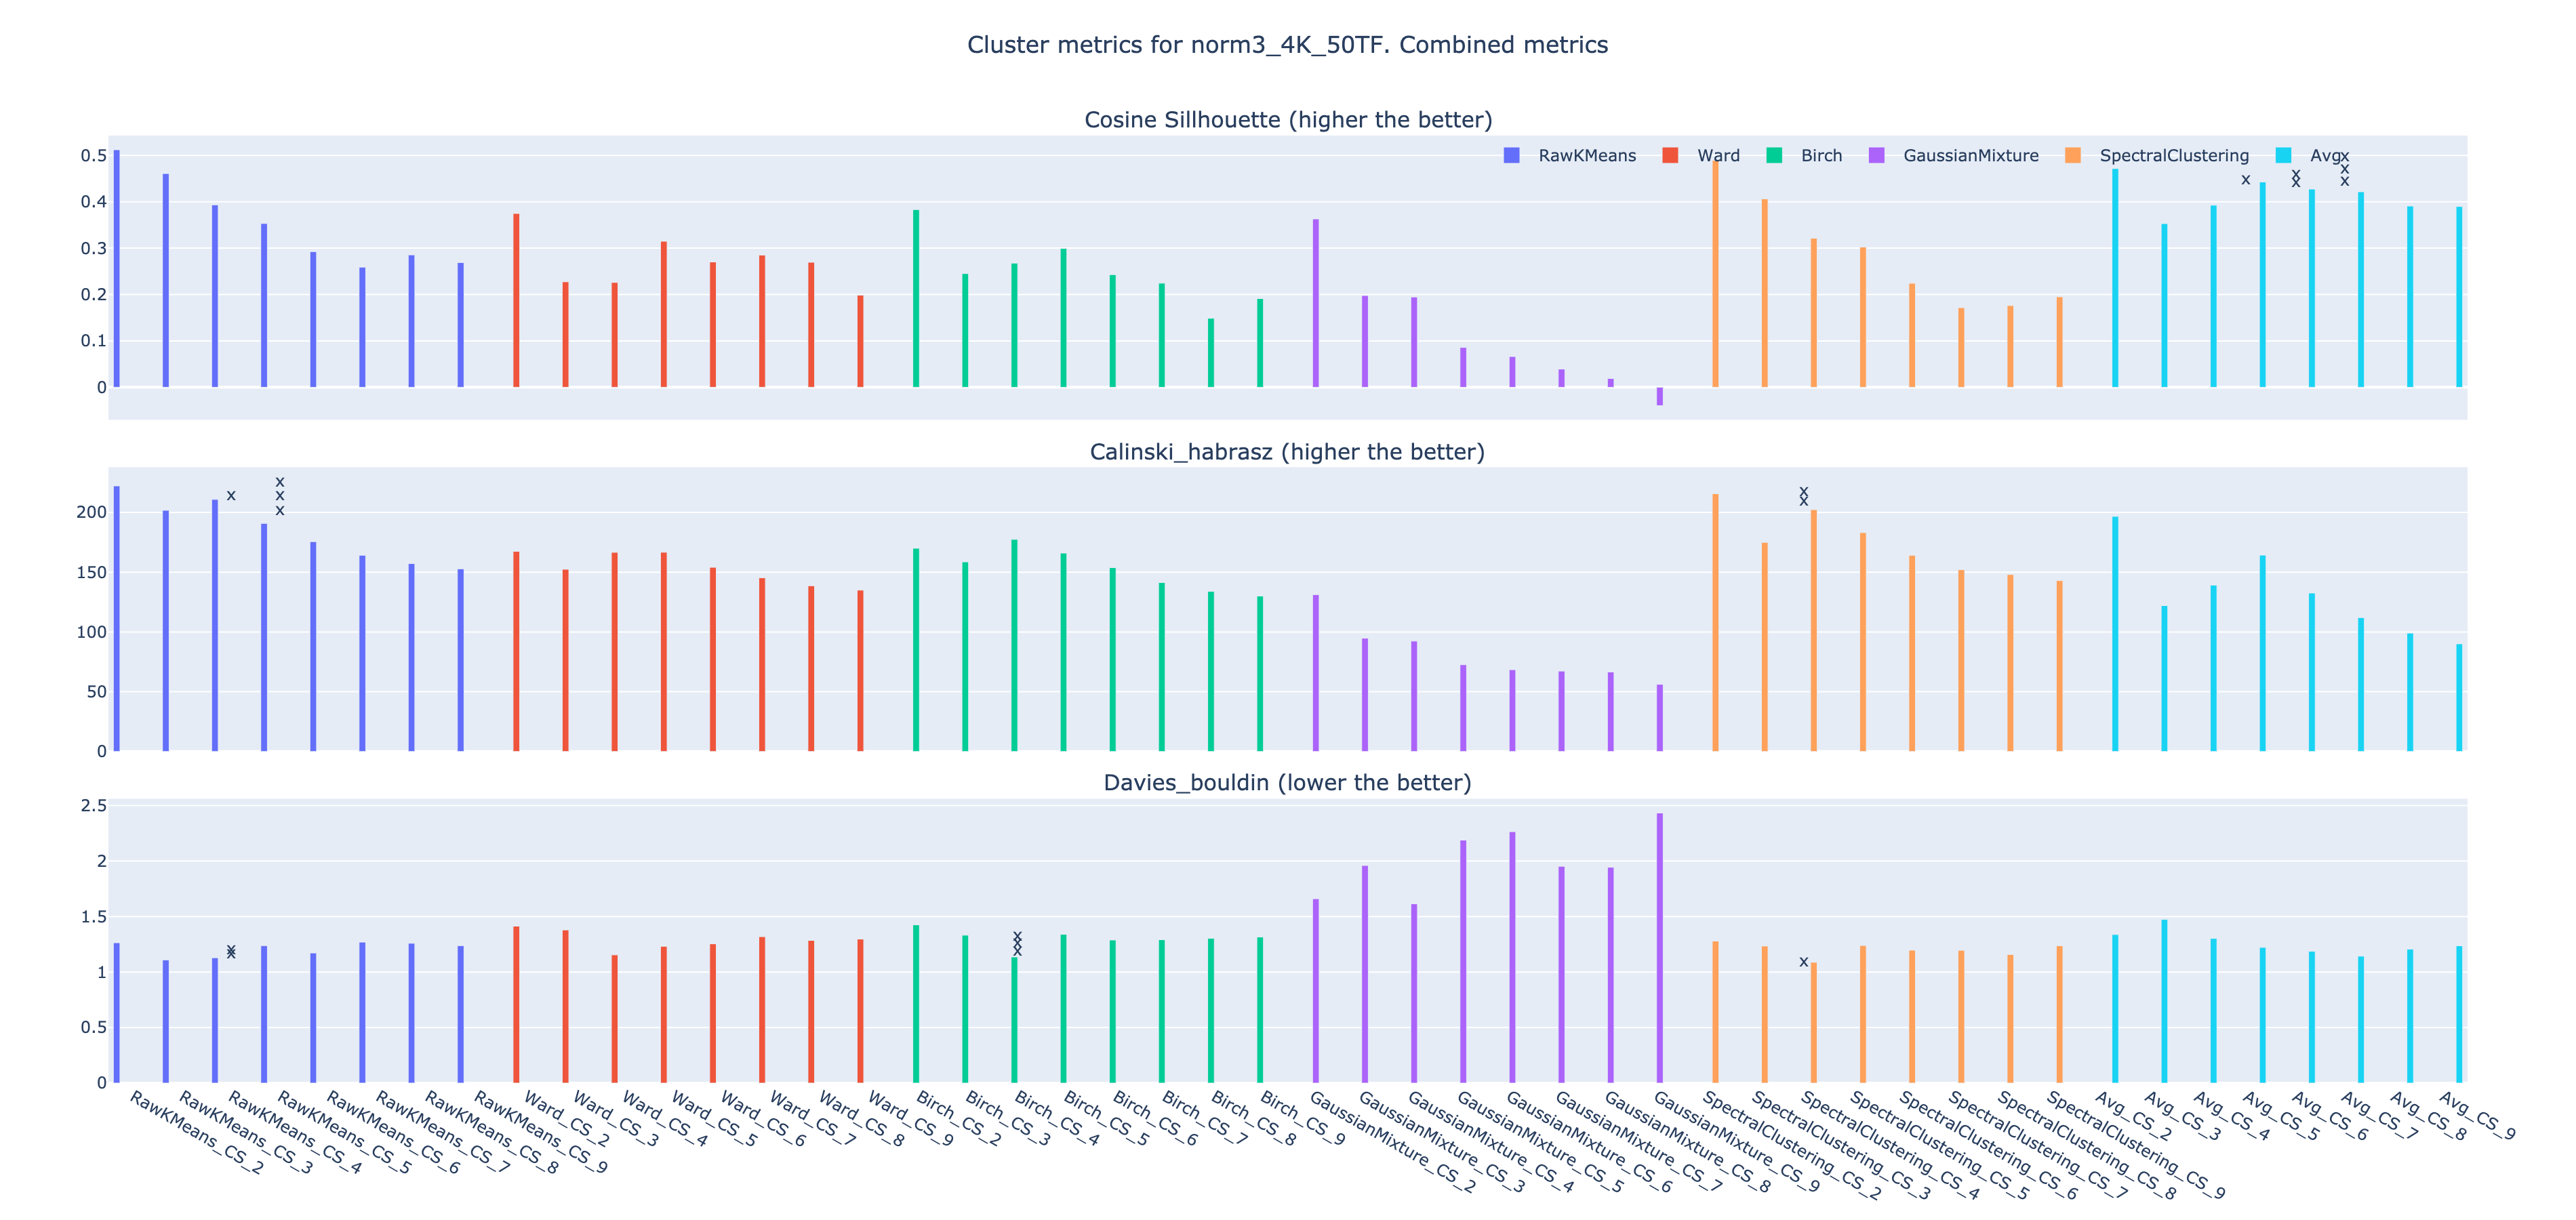
\includegraphics[width=1.0\textwidth,height=0.25\textheight]{Sections/Network_I/Resources/P0/CA_metrics_Rwd_2_tum_4k.png}
        \caption{Reward network}
    \end{subfigure}
    \hfill
    \begin{subfigure}{0.49\linewidth}
        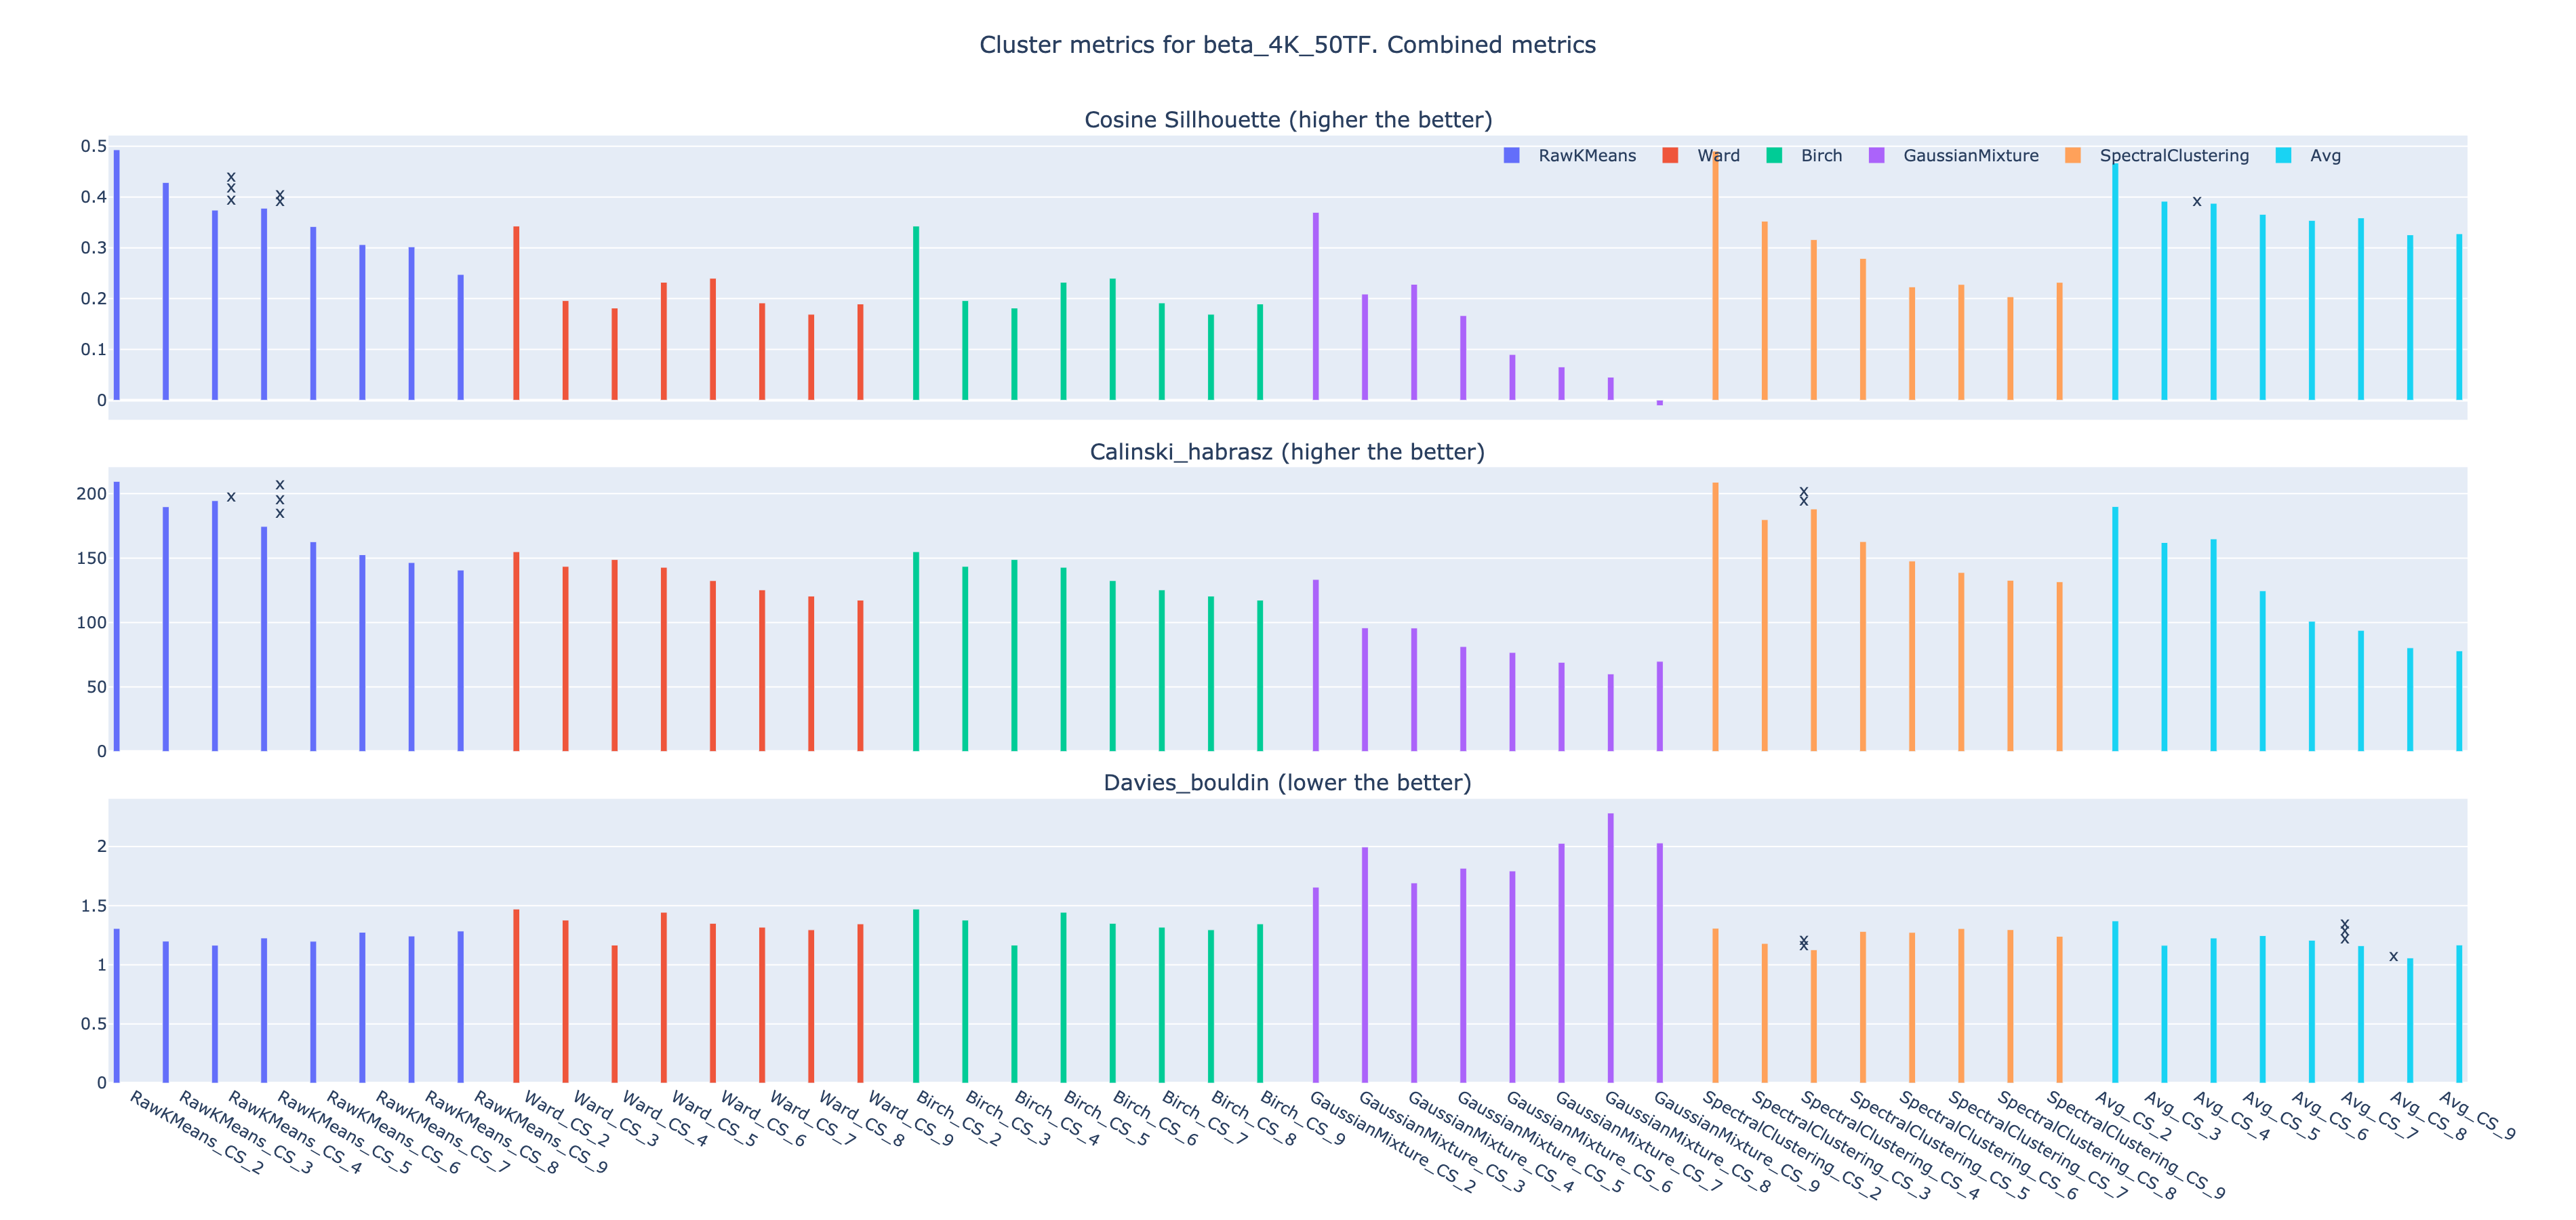
\includegraphics[width=1.0\textwidth,height=0.25\textheight]{Sections/Network_I/Resources/P0/CA_metrics_Pen_2_tum_4k.png}
        \caption{Penalised network}
    \end{subfigure}
    \hfill
    \caption{Clustering metrics for the 3 networks generated from P0 samples.}
    \label{fig:N_I:p0_choosing_cs}
\end{figure}


% Comment on Top 3 models + cs, models and just CS
While Figure \ref{fig:N_I:p0_choosing_cs} shows the general trends of the metrics across the 3 different clustering scores, it is not very clear which model with how many clusters performs the best for each network or overall. Figure \ref{fig:N_I:p0_top_3_metrics} assists the decision making by looking at both the most used cluster model and number of clusters, and separately at the cluster model and size in A), B) and C); the colouring scale corresponds to the encounter frequency across network type; e.g. in A) K-means with K=4 appears 3 times in standard network and Spectral Clustering with K=4 two times in all three network types. The colouring strategies helps delineating the configurations for each network. From Figure \ref{fig:N_I:p0_choosing_cs} A) it can be noticed that the standard network is the only one having a model picked by all three metrics. In B) it is clearer that K-means is the preferred model by both standard and penalised network, while for Reward network both Agg\_Avg and K-means are selected 3 times. In terms of the the cluster sizes, in Figure \ref{fig:N_I:p0_choosing_cs} C), K=4 is the most common number of subgroups followed by K=5. Overall, the clustering scores suggest that both K-Means and Agg\_Avg have similar performances while the preferred cluster sizes is K=4 followed by K=5. Furthermore, K=4 is the overall choice of clusters numbers through the Elbow approach in Figure \ref{fig:N_I:p0_top_3_metrics} D.


% Using cosine sillhouette to look at the spread
The lack of an obvious cluster model shows the challenge of working with gene expression datasets. It also shows the limitation of using average scores for clustering metrics. Thus, we select the Silhouette cosine score\footnote{For the same reason as we chosen it as a main metric in the last chapter. Compared with the other metrics the Silhouette score uses cosine as a distance which is more suitable for high dimension data.} to look at the variance across samples in Figure \ref{fig:N_I:p0_sillhouette_spread}. With the exception of the Agg\_Avg and K-means the other clustering models have a higher spread of the silhouette across the different cluster size.

% narrowing done to the 2 clustering models
The clustering scores and the analysis performed suggests that K-means and Agglomerative Clustering with average linkage perform better than the rest as in the top 3 models used \ref{fig:N_I:p0_top_3_metrics} B) and the silhouette spread in Figure \ref{fig:N_I:p0_sillhouette_spread}. The Elbow method Figure \ref{fig:N_I:p0_top_3_metrics} D) and the other metrics suggests that K=4 is the right choice. This is different from what is expected as in the earlier work \ref{}\footnote{Subtypes section} we found at least five clusters using computational methods and K=6 with biological knowledge (IFNg groups). Also, this is is the next K considered as K=2,3 are not taken in account when finding the top 3 scores as it was explained at the beginning of the section.

\begin{figure}[!htb]
    \hfill
    \begin{subfigure}[b]{0.49\textwidth}
        \centering
        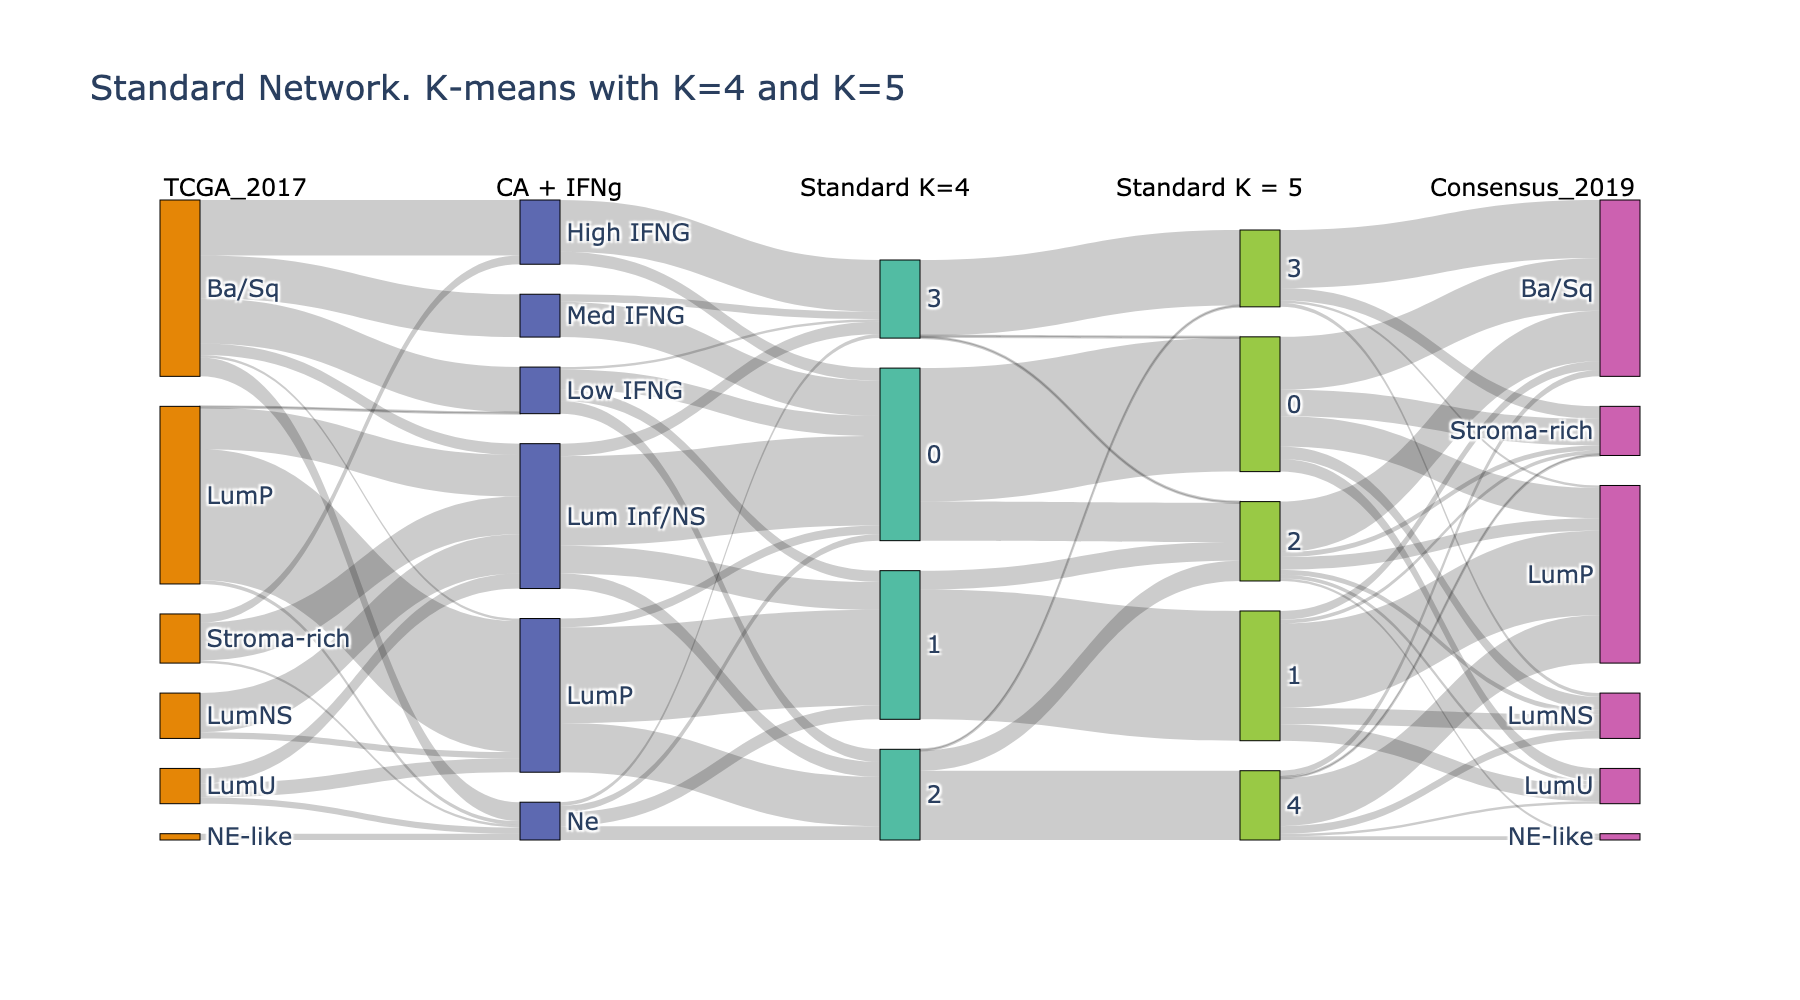
\includegraphics[width=\textwidth,keepaspectratio]{Sections/Network_I/Resources/P0/Sankey_KM_4K.png}
        \caption{K-Means}
    \end{subfigure}
    \hfill
    \begin{subfigure}[b]{0.49\textwidth}
        \centering
        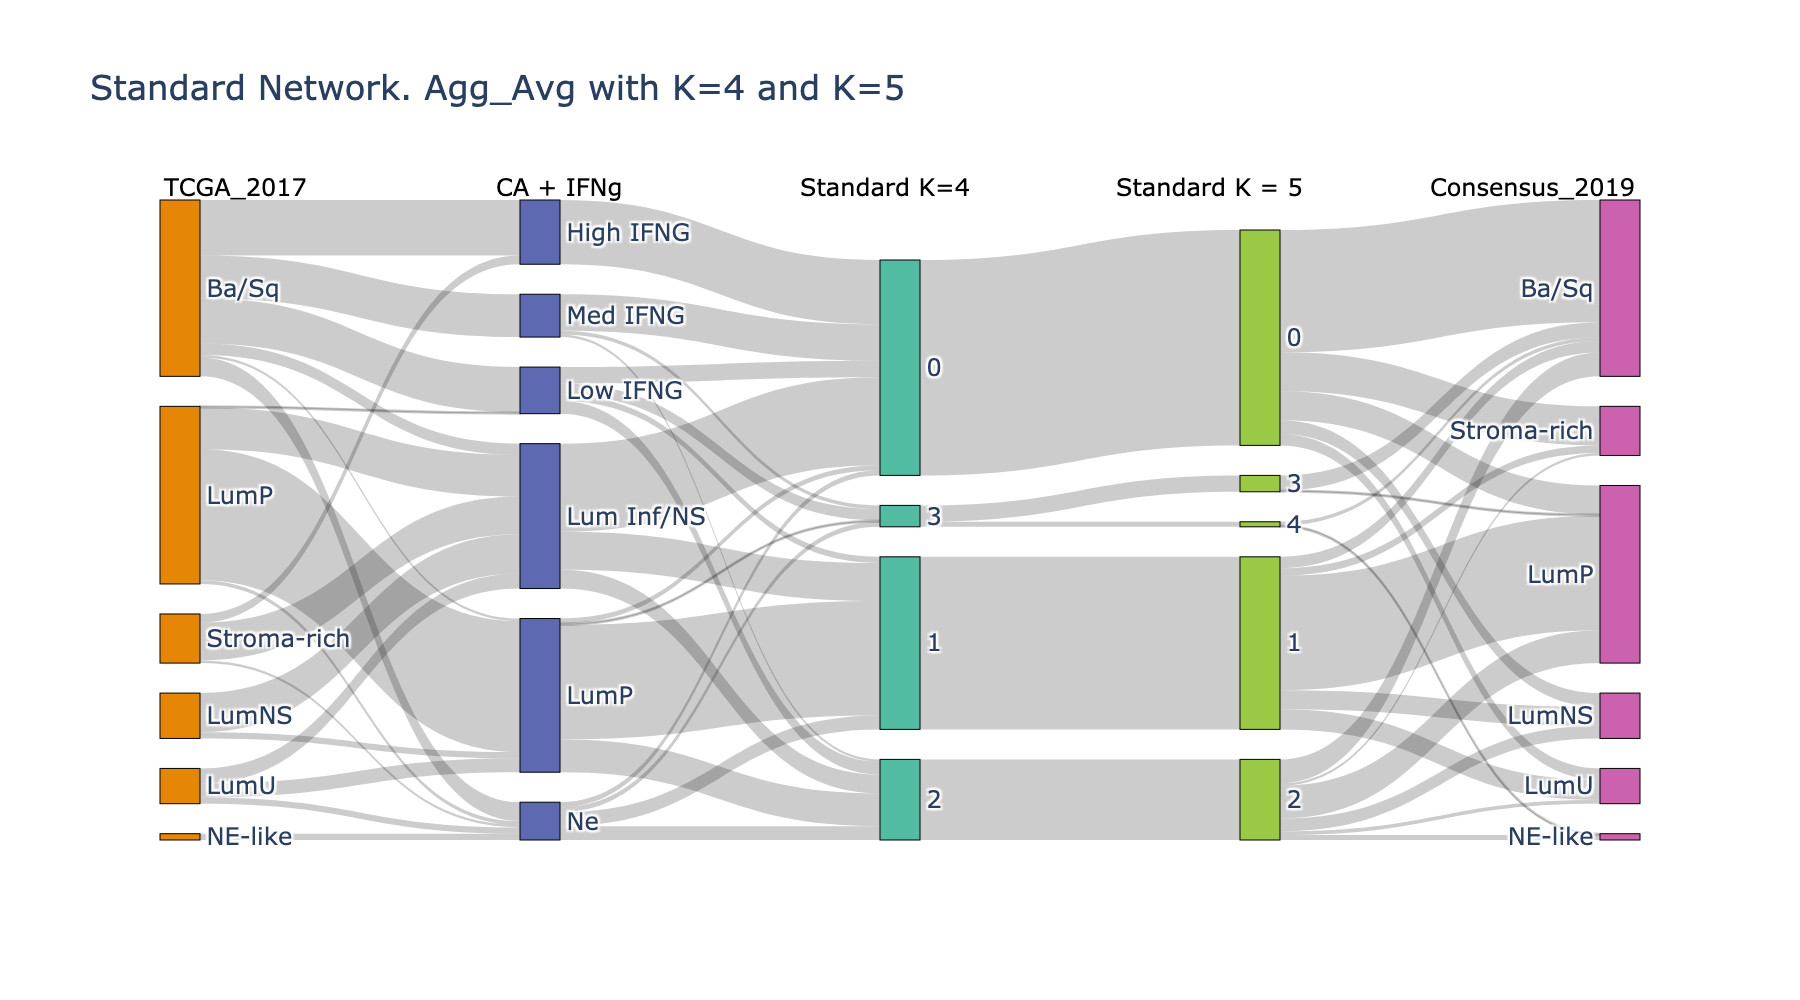
\includegraphics[width=\textwidth,keepaspectratio]{Sections/Network_I/Resources/P0/Sankey_Avg_4K.png}
        \caption{Agglomerative with average linkage}
    \end{subfigure}
    \hfill
    \caption{Sankey plots for the two best performing models. }
    \label{fig:N_I:p0_sky_Agg_KMeans}
\end{figure}


Two Sankey plots in Figure \ref{fig:N_I:p0_sky_Agg_KMeans} are used to assess the differences in the MIBC subtyping between the two best clustering model and the two cluster sizes\footnote{The standard networks were only used for comparison to simplify the process.}. There is a striking difference between the two clustering models, Agg\_Avg finds disproportionate clusters while the K-means finds similar size groups. This, together with the High IFNG subgroup found by K-means suggests that this model is the best choice. 


The cluster metrics are not very useful in determining the number of clusters, the scores decrease proportionally with the number of clusters, thus the best result if given by the lowest K. Elbow method helps in this case but one it is a heuristic approach. In Figure \ref{fig:N_I:p0_sky_Agg_KMeans} A) when K=5, the larger group 0 from K=4 is split into smaller groups, see subtype 2 \& 5 (when K=5). For this and the fact that it is expected to find larger groups K=5 is preferred over K=4.


\subsubsection{Network comparison}


Figure \ref{fig:N_I:p0_sky_leiden} represents an overview of the decisions made in the previous sub-sections, K-means (K=5) was found to be the most suitable clustering model. The three networks are compared with the consensus and TCGA classifiers \citet{Kamoun2020-tj, Robertson2017-mg} as well as our subtyping from Section \ref{}). From the top left figure it can be observed that there number of communities is similar across the three networks, there are 9 or 10 with a few exceptions. There are significantly less communities compared with the number of subgraphs found in the tumour network; see Figure \ref{fig:N_I:tum_leiden_modifiers}. The small variance of the Modularity score in the Figure on the right suggests that the communities are fairly stable and the penalised network have a lower performance by 0.04.

\begin{figure}[!htb]    
    \centering
    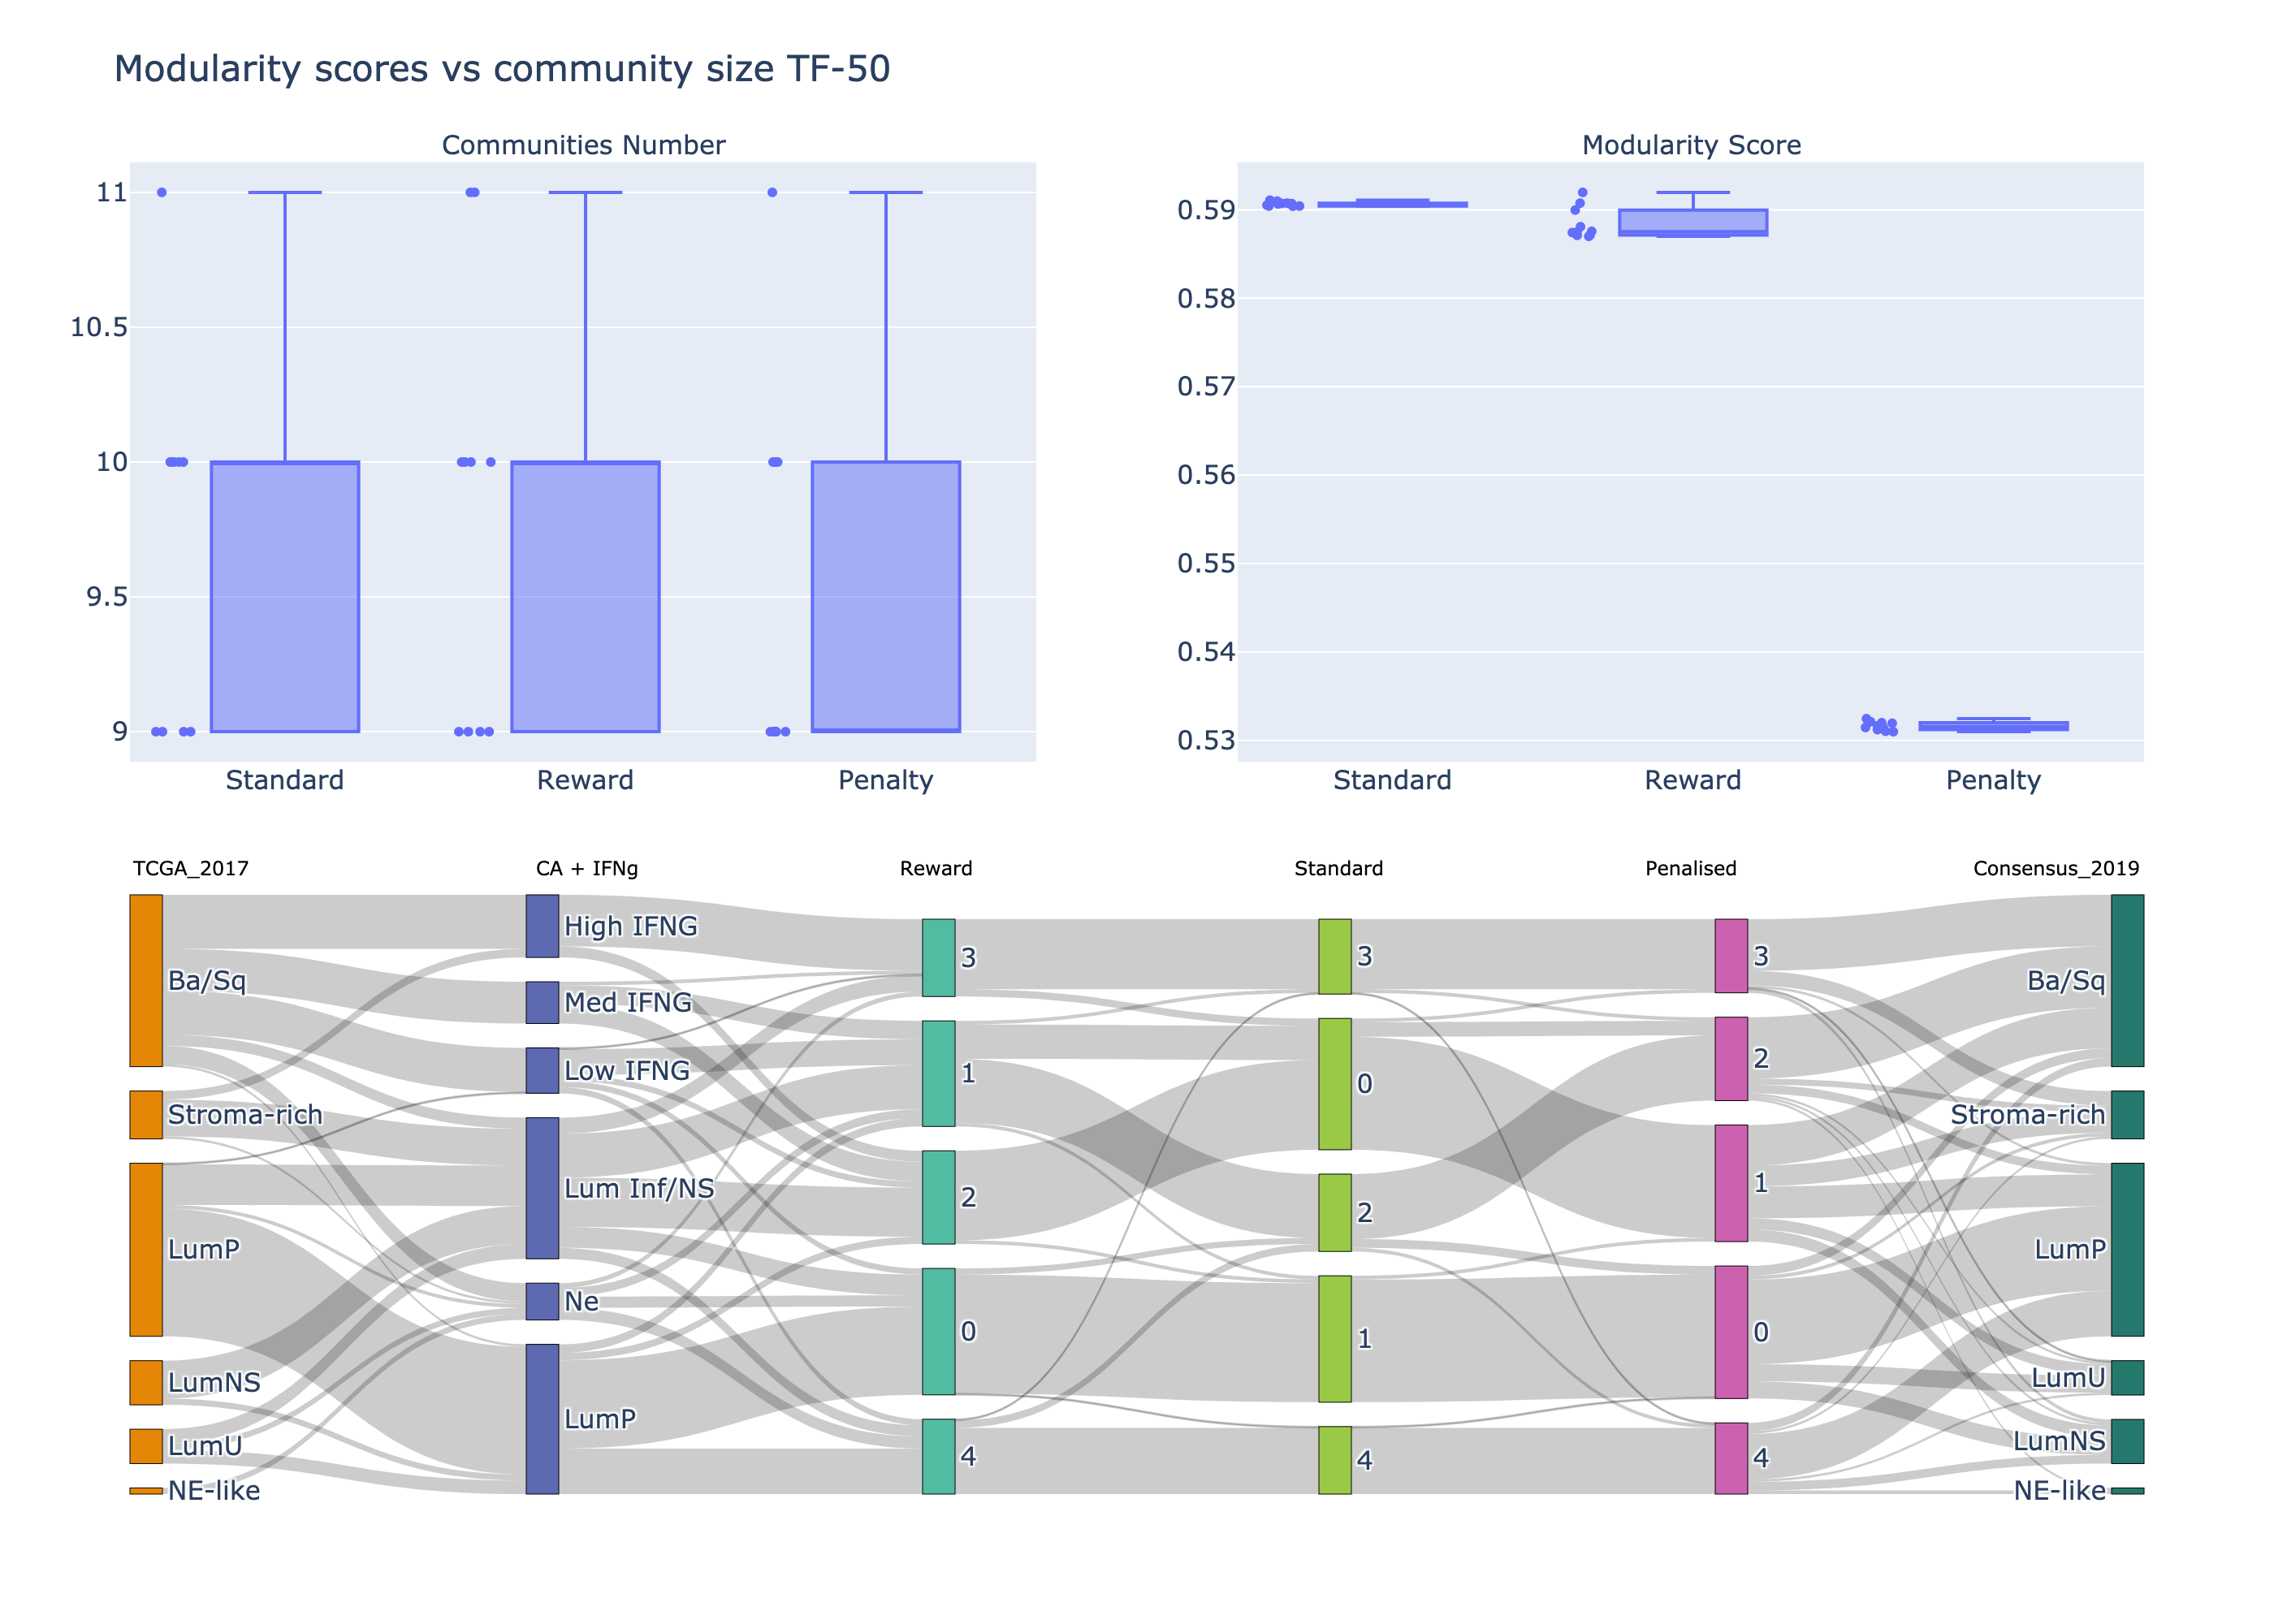
\includegraphics[width=1.0\textwidth,height=0.7\textheight,keepaspectratio]{Sections/Network_I/Resources/P0/Ldn_Sky_TF_50_RawKMeans_K5.png}
    \caption{Overview of the MIBC stratification using P0 dataset.}
    \label{fig:N_I:p0_sky_leiden}
\end{figure}

From the Sankey plot it can be seen that the High IFNG group (CA+IFNg) is contained across the 3 networks in cluster 3. Groups 2 in Standard and Penalised are similar and formed mostly from Ba/Sq groups while cluster 1 (Reward) has additional samples from LumInf/NS\footnote{Would this mean that by increasing the weight values more samples are added to the group? While pruning edges removes some of the noise?}. The cluster 0 from the Standard network resembles to the LumInf/NS group from the CA+IFNG classification, being a mixed of samples. Group 0 (Reward and Penalised) and 1 (Standard) contains samples which previously were considered Luminal samples. Lastly, cluster 4 contains a consistent number of samples which previously classified as LumP or/and Luminal Unstable (LumU), Unspecified (LumNS).

Overall, the comparison between classifications shows that the network approaches exhibit different subtypes from the other traditional methods. Several samples change group membership in the three different networks, but there are no large changes. This suggests that the weight modifiers strategies have little effect on the subtyping.

\subsubsection{Community analysis}

Previous results with tumour networks (Section \ref{s:N_I:tum}) showed that the weight modifiers do have an effect on the network metrics but little effect on the MIBC subtyping. A natural next step is to analyse the changes in communities when a modifier is applied. There are a few questions to answers 1) How do the communities change? 2) Is there a difference in mutation burden? 3) How much the gene expression differs? 

\begin{figure}[!htb]
    \hfill
    \begin{subfigure}[b]{0.49\textwidth}
        \centering
        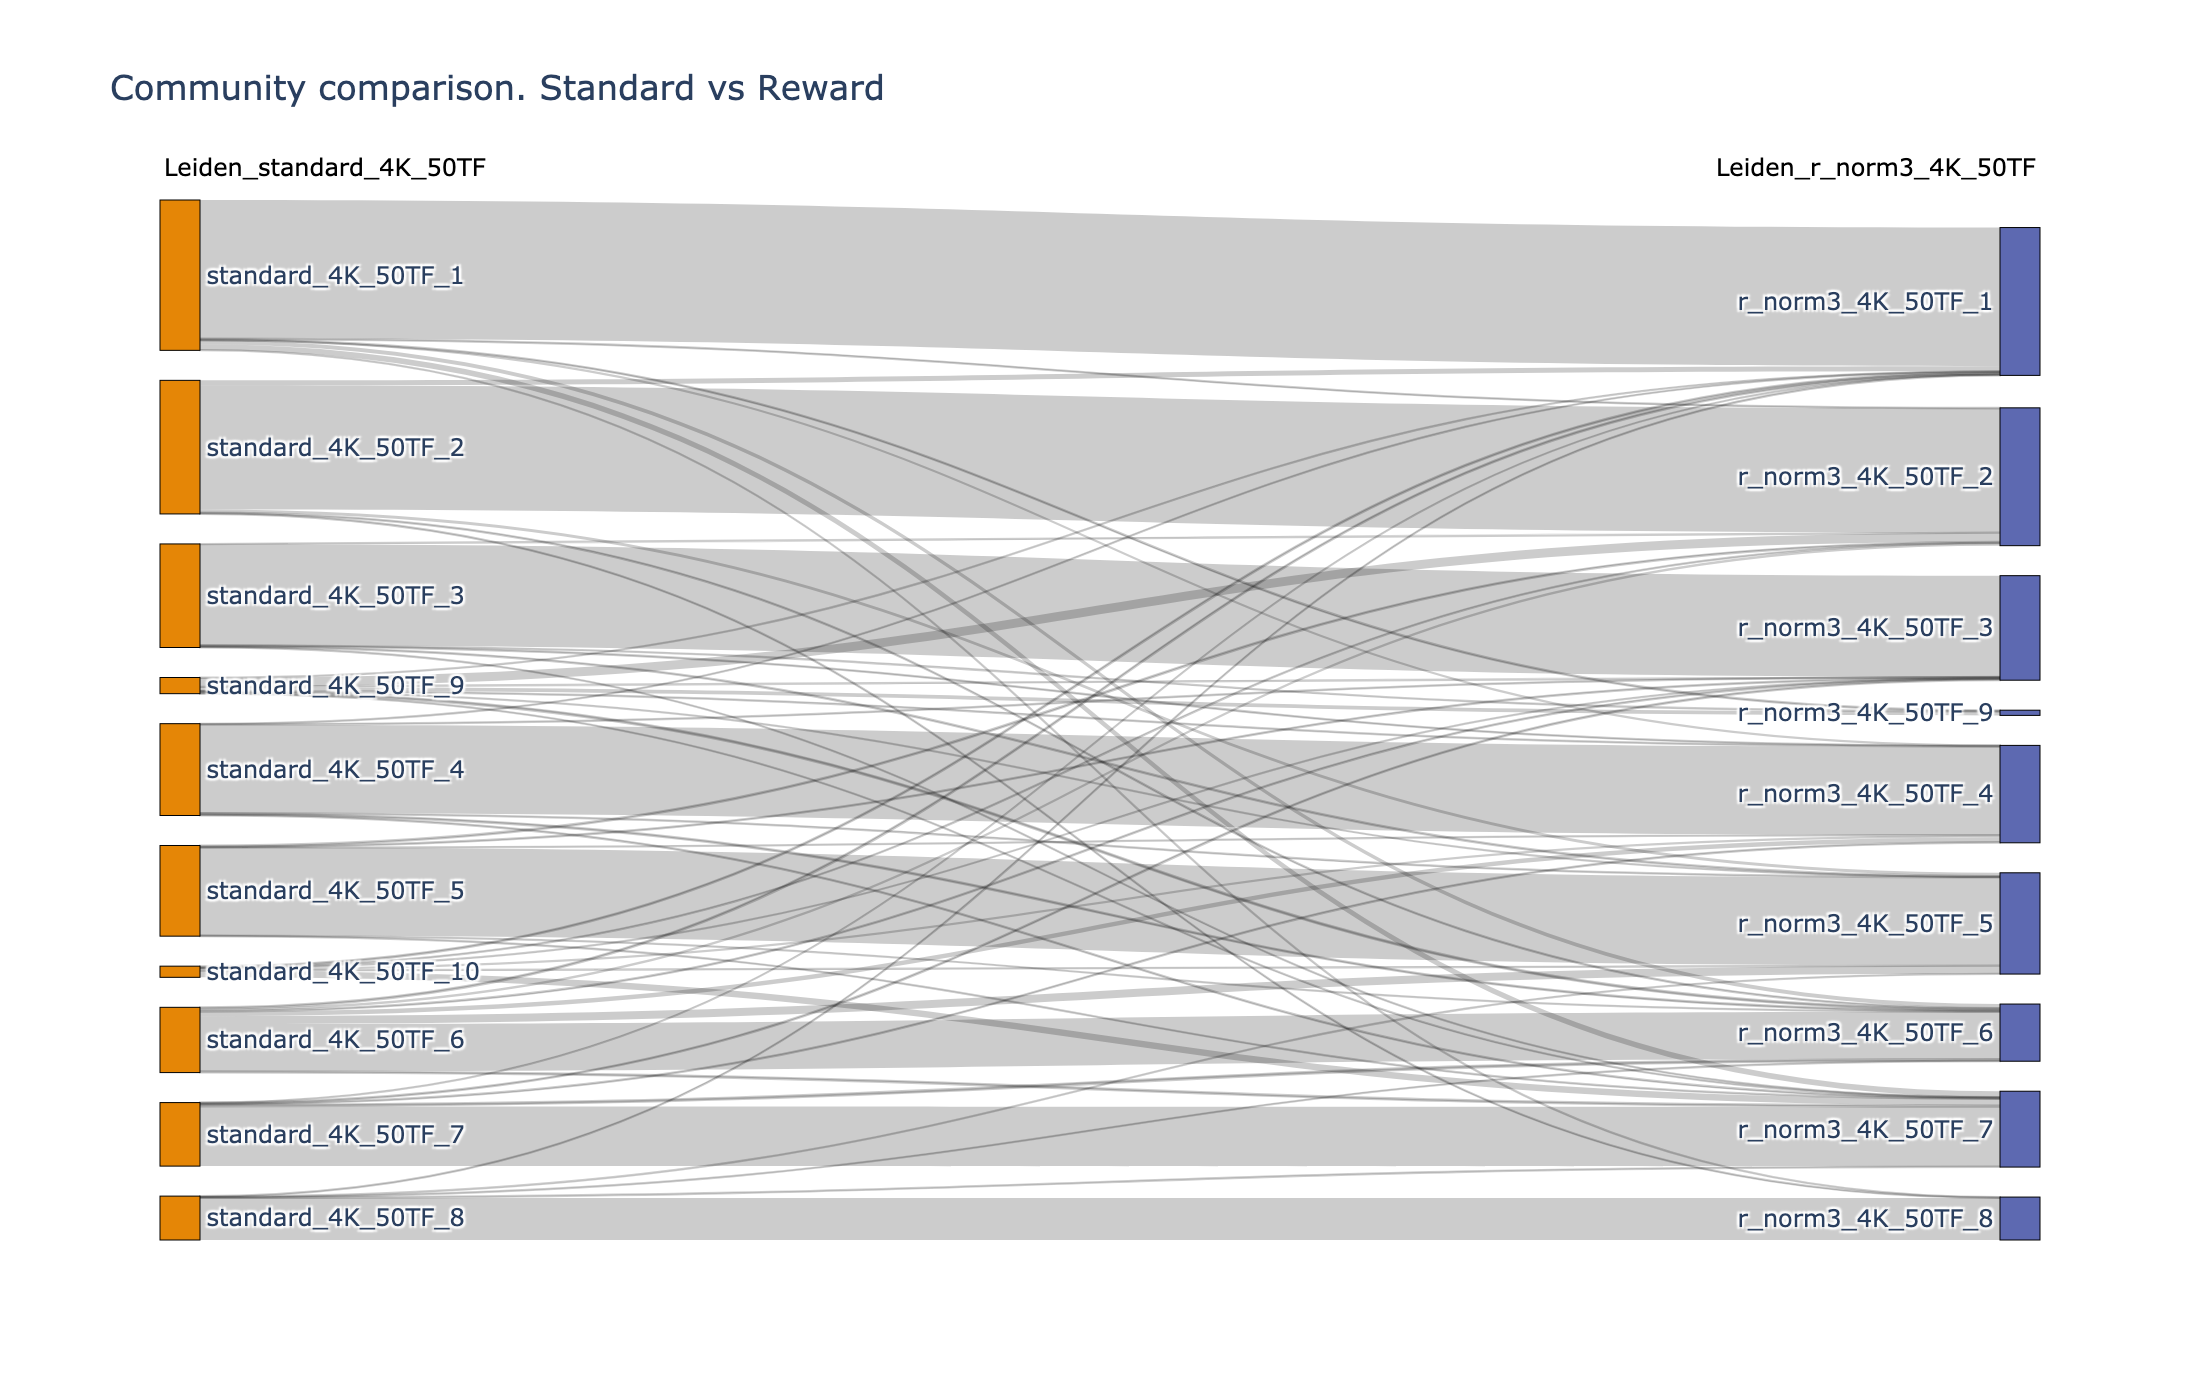
\includegraphics[width=\textwidth,keepaspectratio]{Sections/Network_I/Resources/P0/Comms/Sky_Comm_Comp_4K.png}
        \caption{Gene changes}
    \end{subfigure}
    \hfill
     \begin{subfigure}[b]{0.49\textwidth}
            \centering
            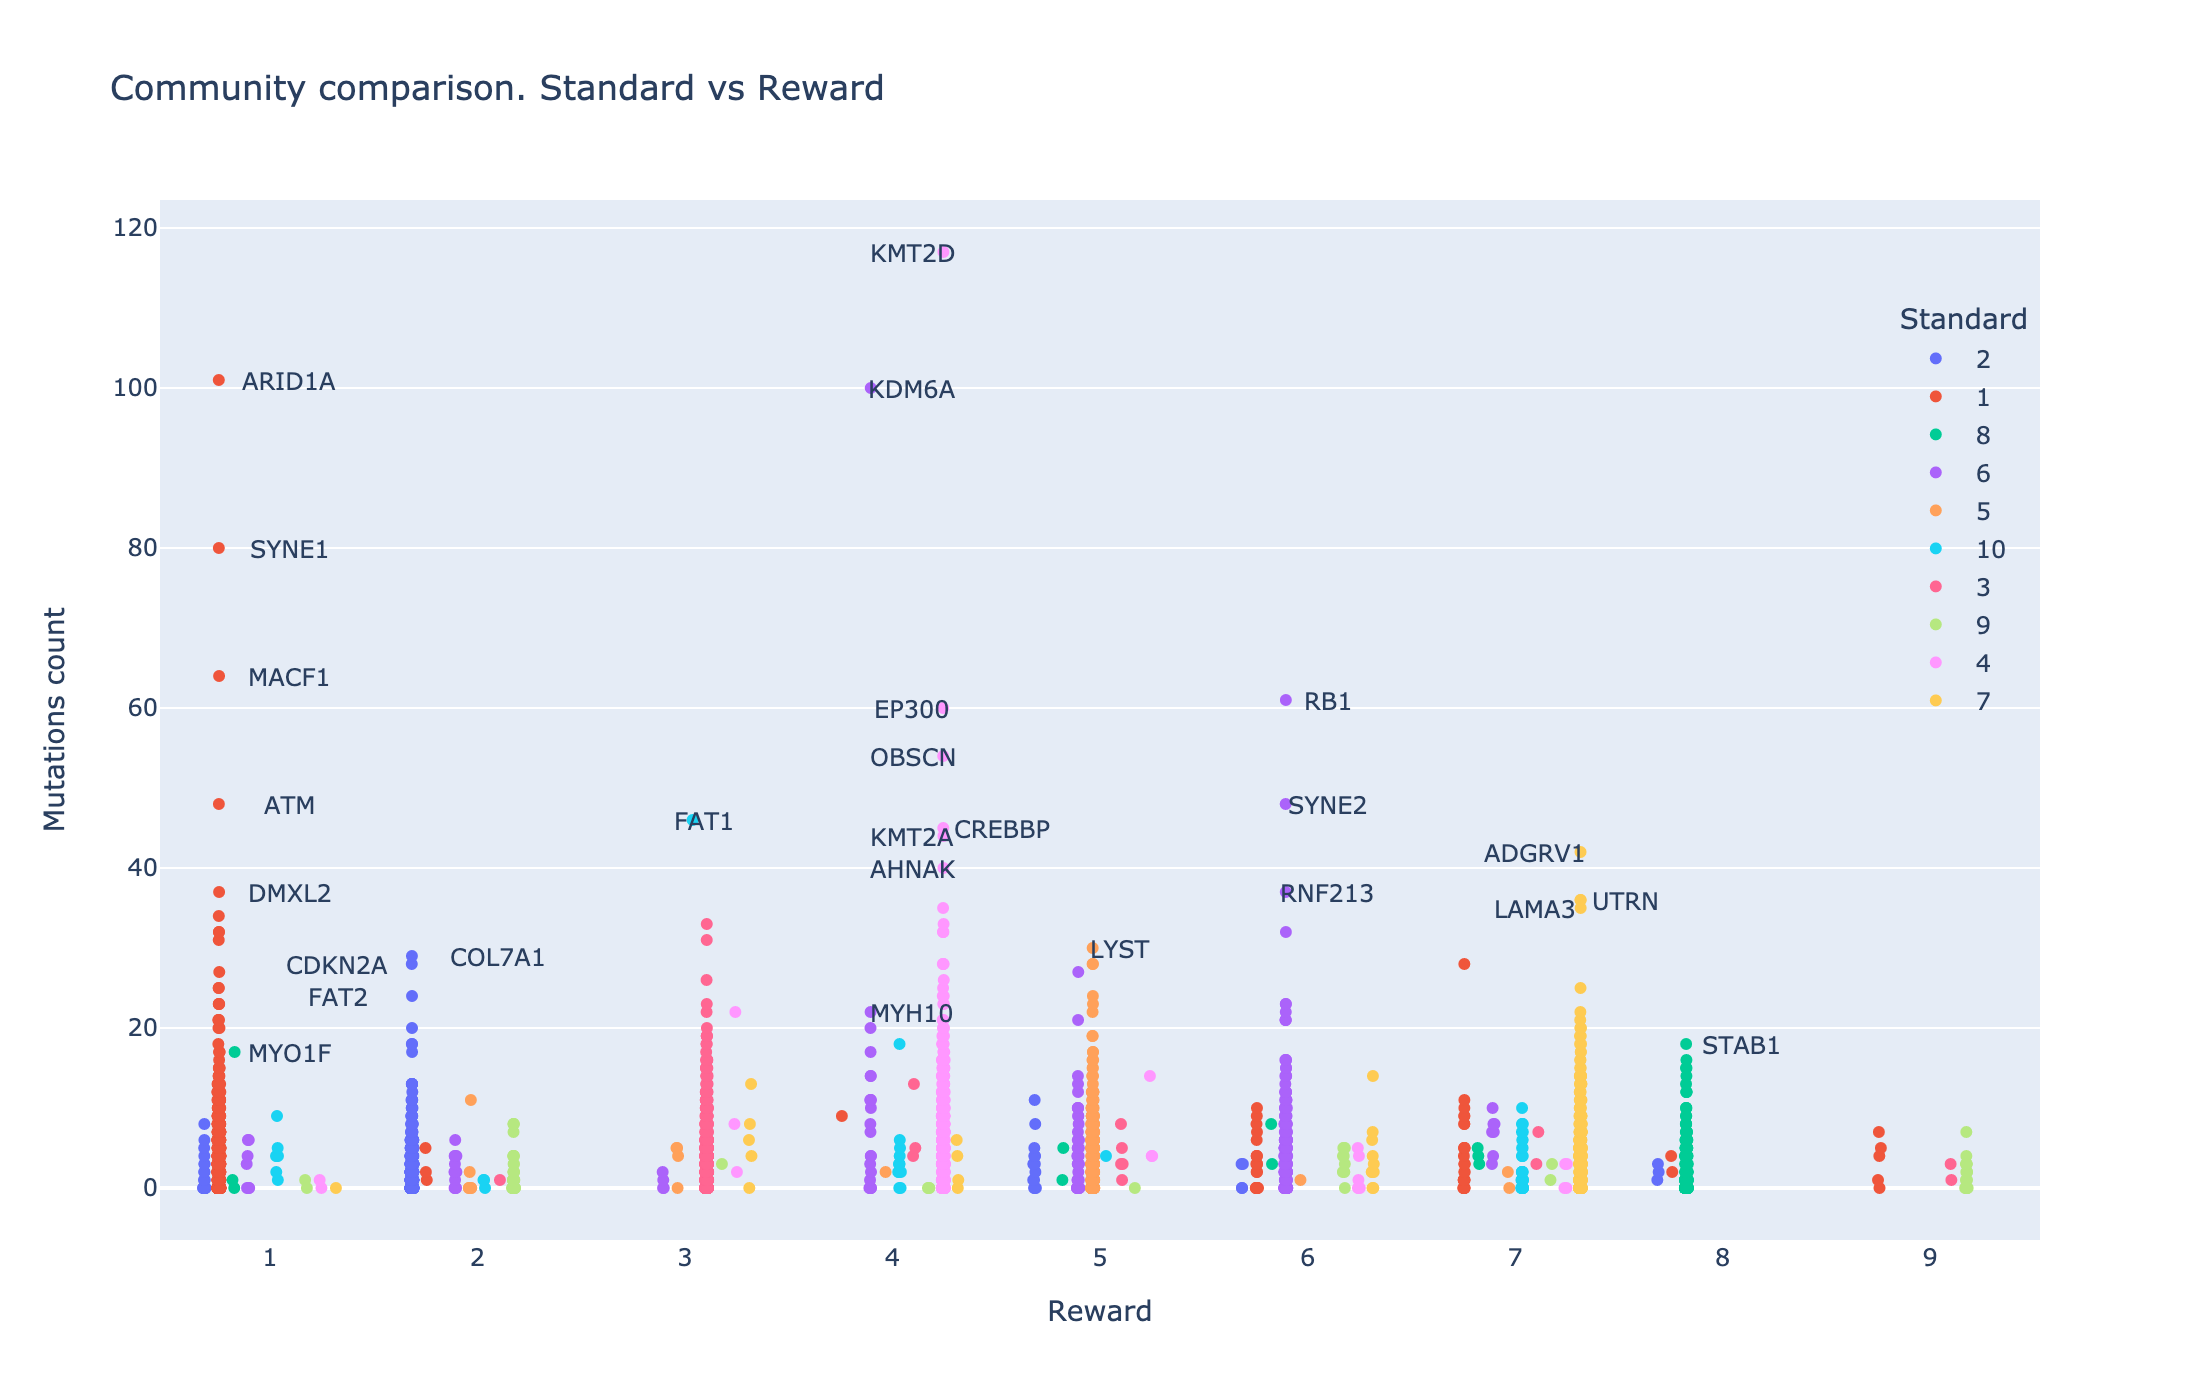
\includegraphics[width=\textwidth,keepaspectratio]{Sections/Network_I/Resources/P0/Comms/Mut_Comm_Comp_4K.png}
            \caption{Mutation representation}
    \end{subfigure}
    \hfill
    \hfill
    \begin{subfigure}[b]{0.47\textwidth}
        \centering
        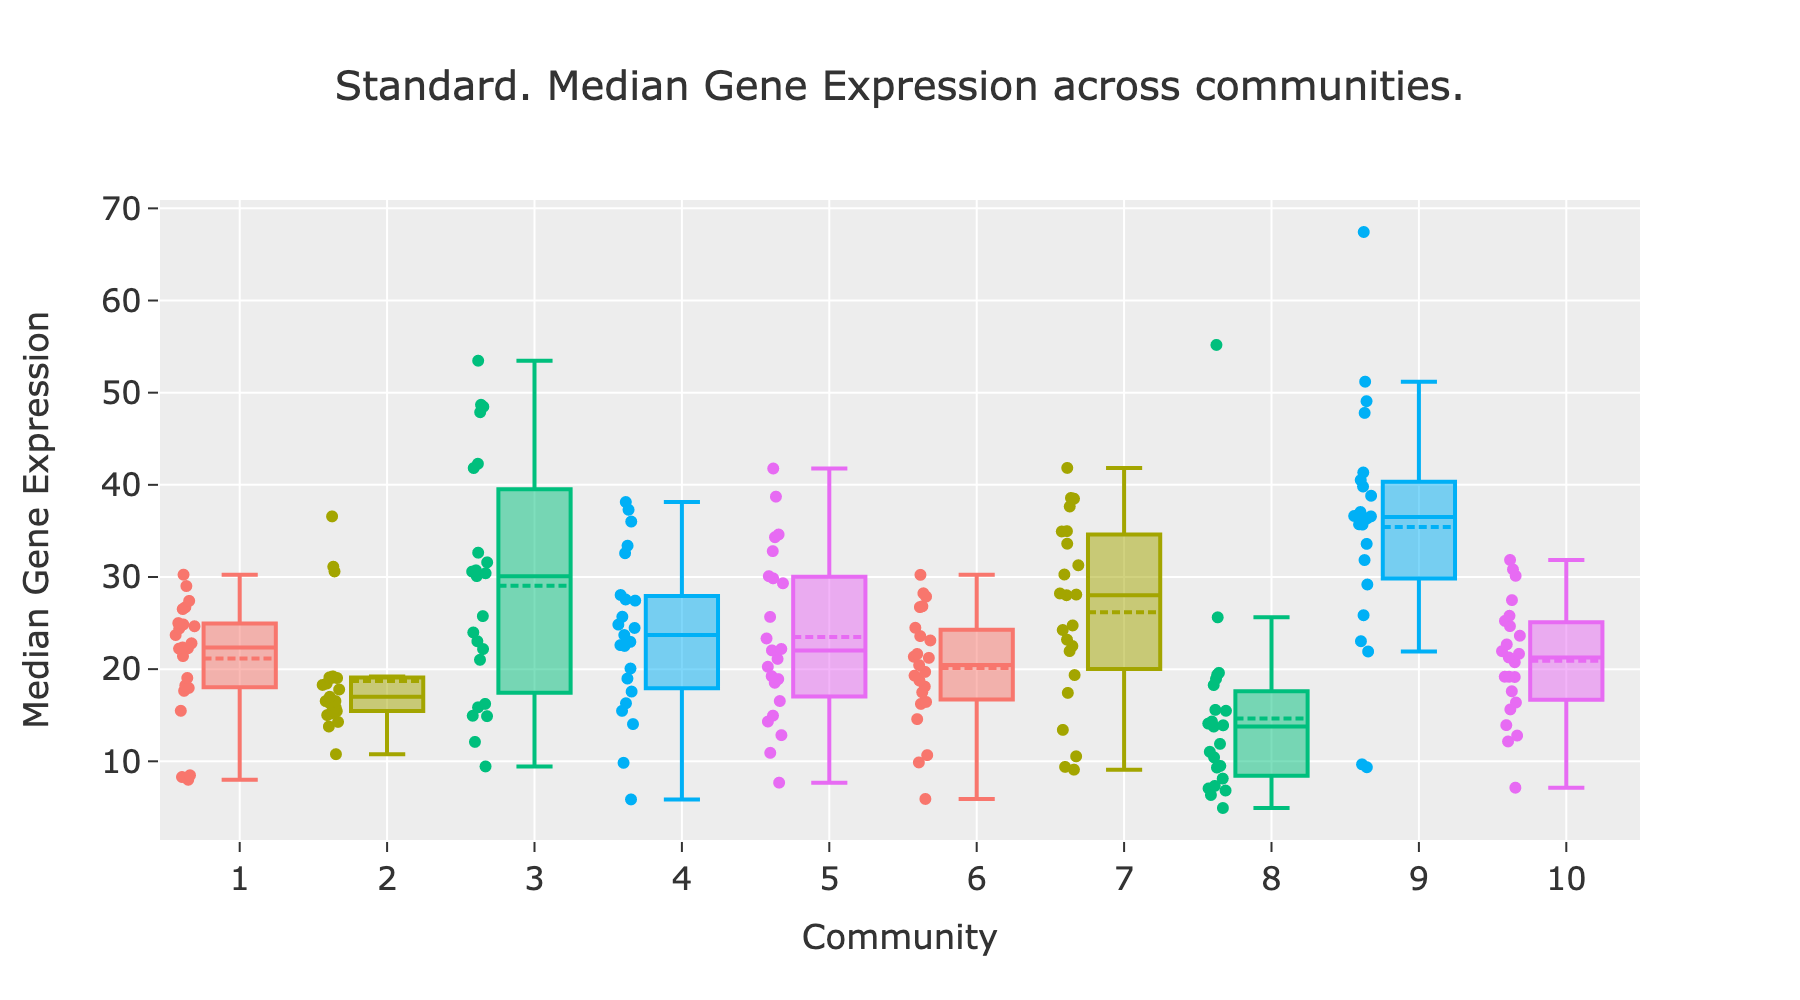
\includegraphics[width=\textwidth,keepaspectratio]{Sections/Network_I/Resources/P0/Comms/P0_standard_4K_50TF_med.png}
        \caption{Standard expression values}
    \end{subfigure}
    \hfill
    \begin{subfigure}[b]{0.47\textwidth}
        \centering
        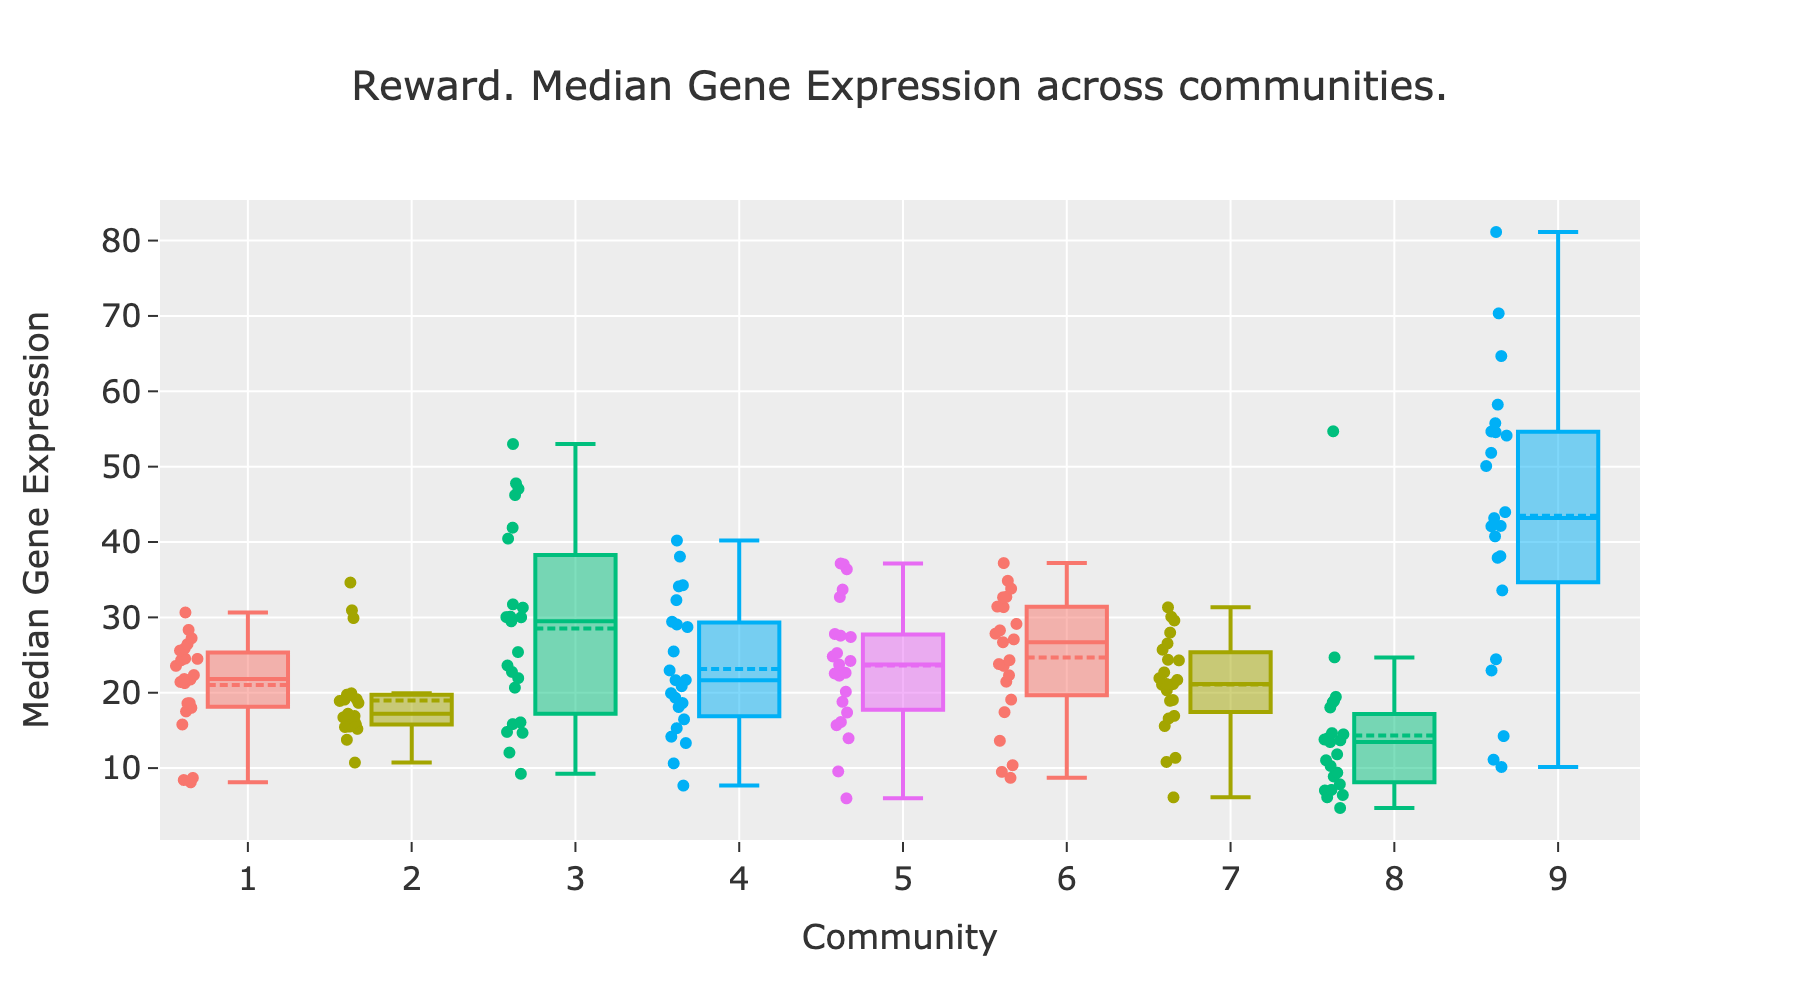
\includegraphics[width=\textwidth,keepaspectratio]{Sections/Network_I/Resources/P0/Comms/P0_norm3_4K_50TF_med.png}
        \caption{Reward expression values}
    \end{subfigure}
    \hfill
    \caption{Gene communities changes.}
    \label{fig:N_I:p0_comm_chgs}
\end{figure}


% How the communities are sincronise
To ease the analysis and based on the Modularity Score, the standard and reward networks are selected for community comparisons. A common problem in unsupervised learning is the group labelling differences between the different models and the standard strategy is to count up from the largest group. This means that there are community labelling differences between the standard and reward networks which makes the analysis confusing. Therefore, the community labels are synchronised to match which is achieved by selecting the standard network as a reference for community numbering. Next, each community in the standard network is matched with the community with the highest representation (i.e. number of genes) from the reward network, this then takes the label from the reference labeling.

% Reward modifier is not powerful enough
Figure \ref{fig:N_I:p0_comm_chgs} sheds some light on the above questions. The sankey in A) shows 
how the genes change communities from the standard to the reward network. The biggest change is represented by the lack of community 10 in the reward network, otherwise the communities remarkable simillar. Figures \ref{fig:N_I:p0_comm_chgs} C), D) show the median gene expression across the communities for the two networks. Communities 1 and two are almost unchanged in the reward network while in the others the spread of the median expression is affected. The most striking difference is in community 9 and 3.  

Figure \ref{fig:N_I:p0_comm_chgs} B) displays the number of mutated genes (Y) in each reward network's community. For each group it can be usually notice that the there are a large number of mutated genes from the same community. Community 1 has a large number of mutations in the standard network and it receives a few more mutated genes from com 2 (standard). Community 4 has lots of mutated genes in the standard but it receives a few from com 6 as well. Communities 8 and 9 have few mutated genes which can be impart explained by their relative small size. Overall, the reward modifier is the trigger of the community changes but it is not powerful enough to set off large community migrations.

% 
Figure \ref{fig:N_I:p0_comm_chgs} B) is a suitable plot to show that most communities have a higher number of mutated genes between the weight modifiers, but it is not suitable too check if the reward modifier affected the genes with the higher mutation burden. Thus, are the genes with the highest mutation count grouped together? In Figure \ref{fig:N_I:p0_mut} it shows the mutation burden across communities. In the standard, communities 1, 2, 3, 4 and 5 have the highest number of genes mutated and it can be noticed that all have the same trend a sharp decline after mutation burden >1; community 4 having the highest number of highly mutated genes. Similar trends can be noticed in the reward network but communities 2,3,4 have a similar slope. In addition, community 9 has just a few mutation with low burden, while 6 and 7 are better separated in the reward. This changes suggests that the highly mutated genes are the ones changing communities.



\begin{figure}[!htb]
    \hfill
    \begin{subfigure}[b]{0.49\textwidth}
        \centering
        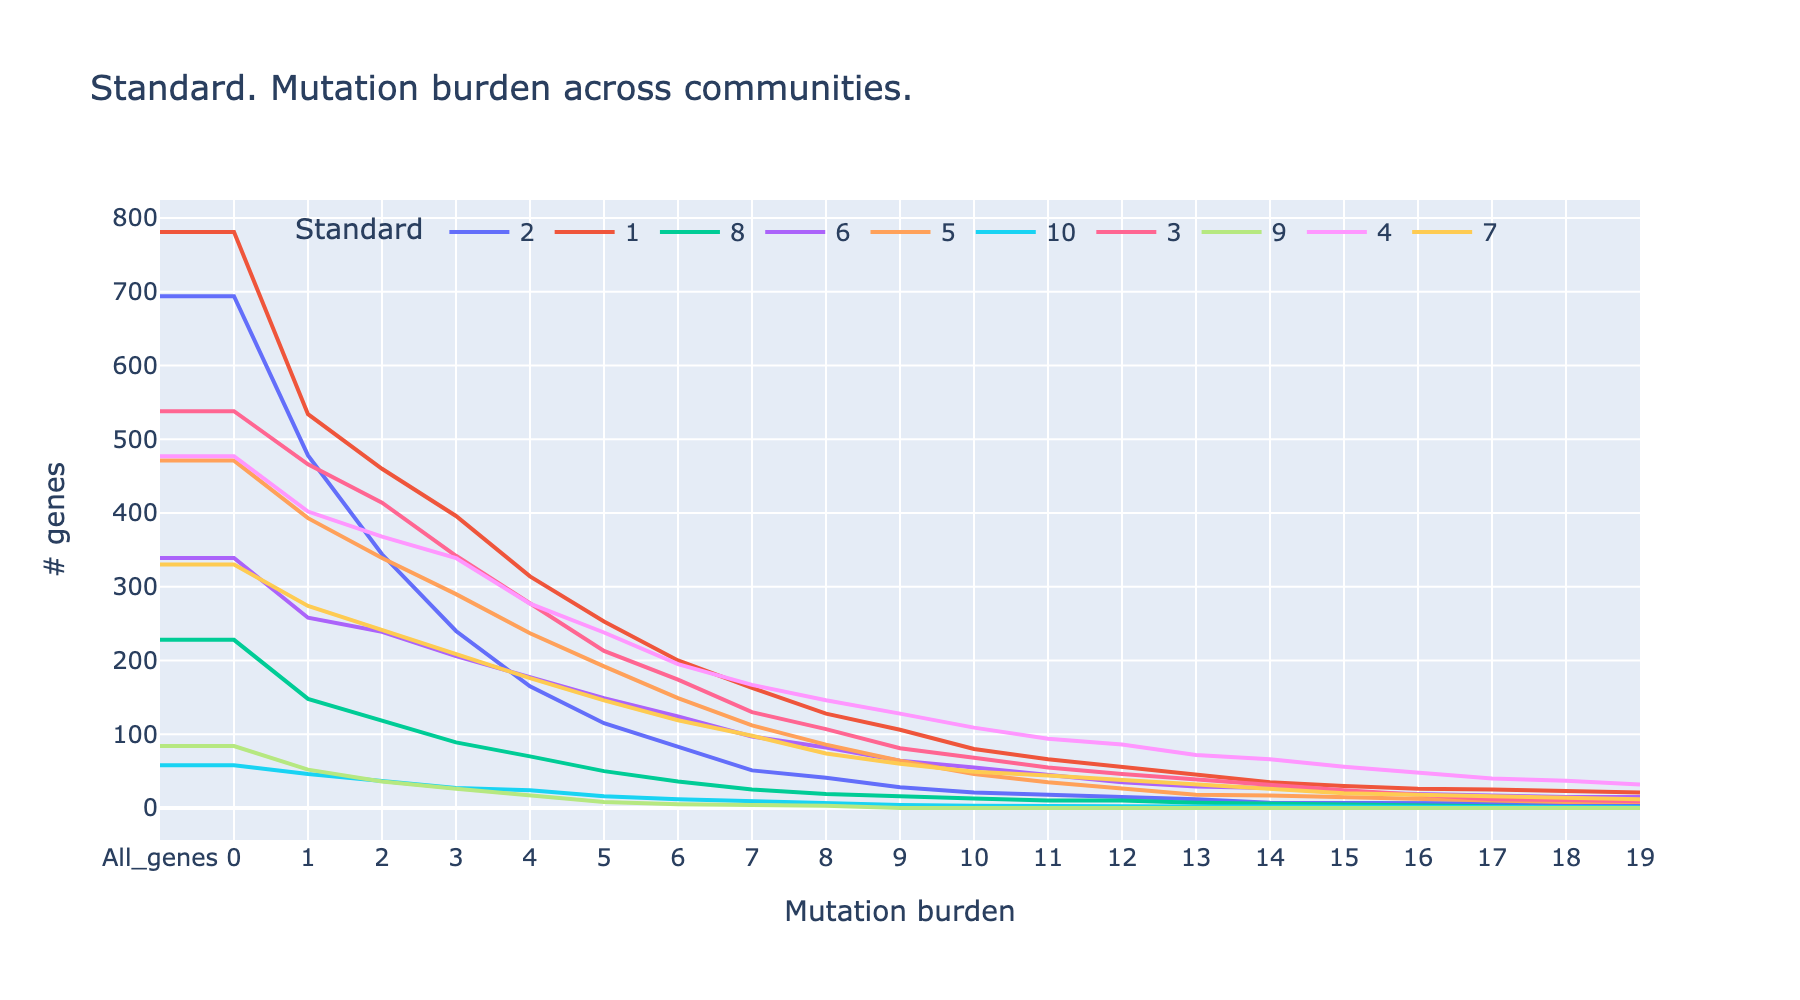
\includegraphics[width=\textwidth,keepaspectratio]{Sections/Network_I/Resources/P0/Comms/Mut_evo_Std_4k.png}
        \caption{Standard}
    \end{subfigure}
    \begin{subfigure}[b]{0.49\textwidth}
        \centering
        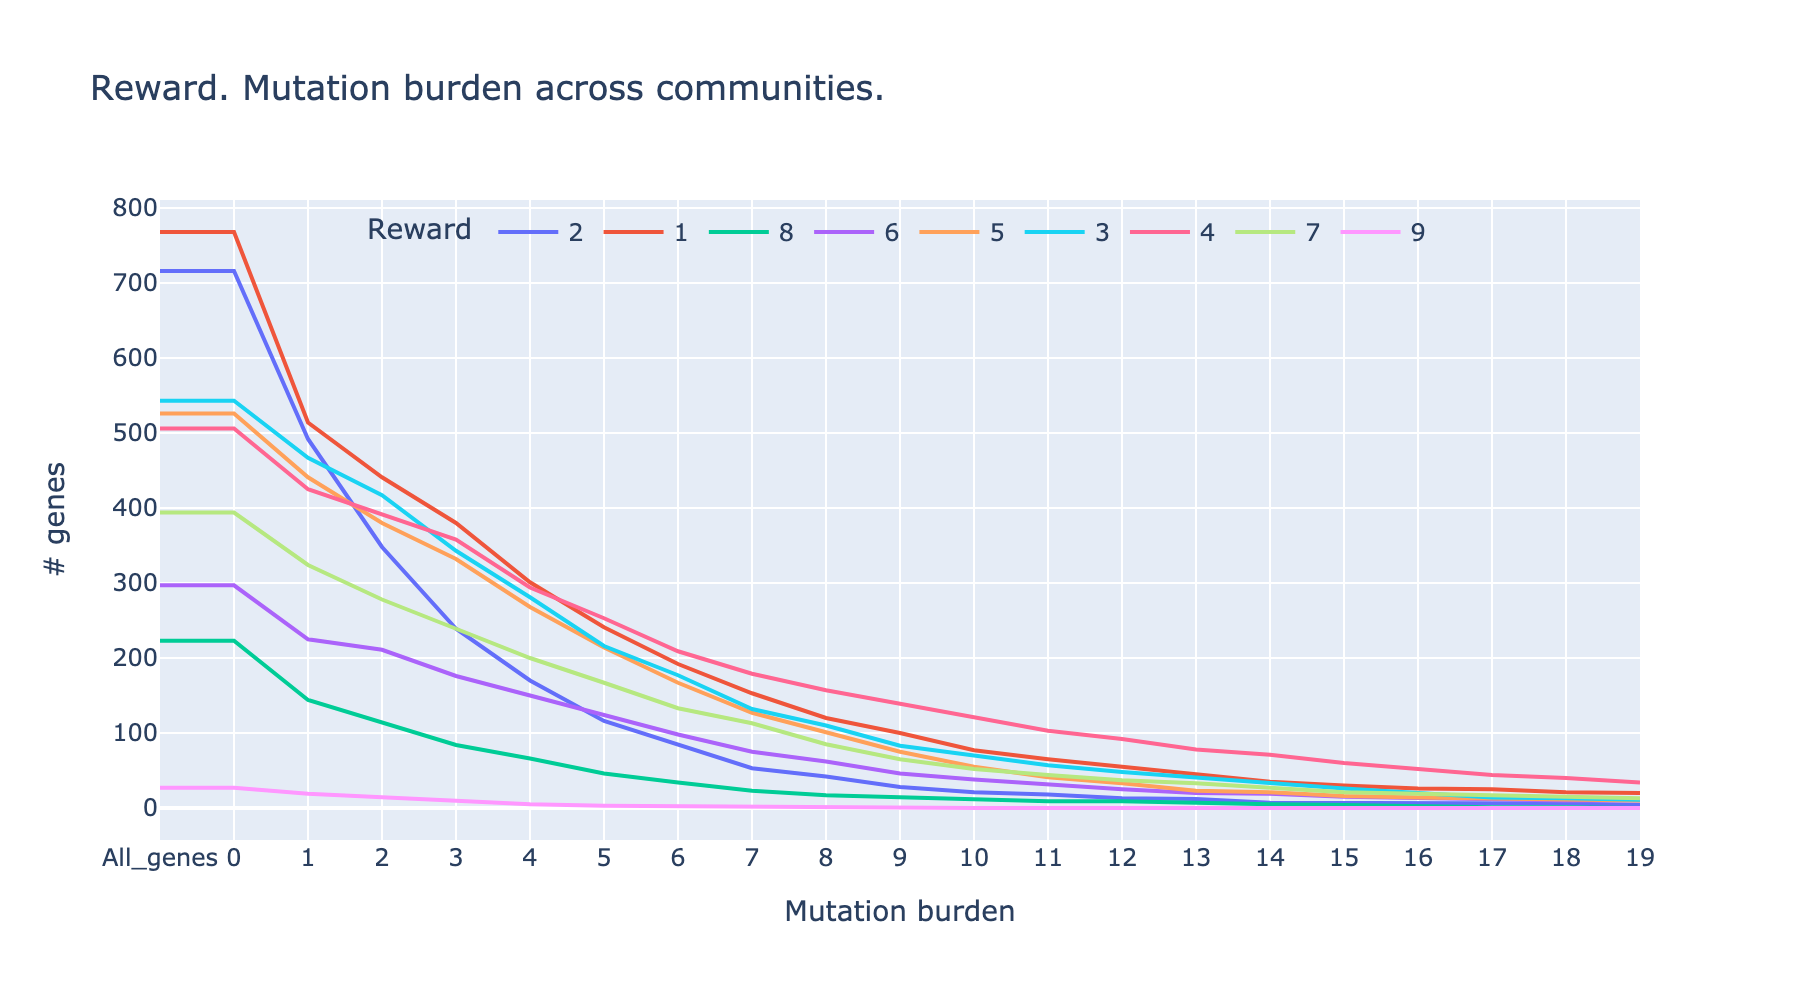
\includegraphics[width=\textwidth,keepaspectratio]{Sections/Network_I/Resources/P0/Comms/Mut_evo_Rwd_4k.png}
        \caption{Reward}
    \end{subfigure}
    \caption{Mutation burden per communities}
    \label{fig:N_I:p0_mut_burden}
\end{figure}


% Conclusion 1 - Weight modifiers work
Overall, the community analysis shows that there reward modifier works, there are changes between communities and this is given by the mutated genes, especially the ones with a high burden. However, the modifier does not have enough power to cause large changes.

\subsubsection{Gene representation}

It is worth remembering that the network is built on the P0 data and then the information extracted from there it is used to stratify the tumour dataset. The two types of data is expected to have differences in gene expression, some of the genes may be expressed in the P0 data but not in the tumour and vice-versa. Therefore, it is important to understand how well the genes selected are represented through the network approach (ModCon and MEV) in the tumour dataset. 


% Conclusion 2 - Poor representation
Figure \ref{fig:N_I:p0_mev_rep} shows that representation for each community. In Figure \ref{fig:N_I:p0_mev_rep} A) shows the genes selected are represented in the most varied genes (in TCGA) while B) in all the expressed genes. From the two sub-figures it can be clearly seen that using just the most varied genes was missing a large number of genes. Nevertheless, there are is still a few genes missing when all the expressed genes are used. This may suggests that using a larger dataset may help increase the gene coverage. 

\begin{figure}[!htb]
    \hfill
    \begin{subfigure}[b]{0.47\textwidth}
        \centering
        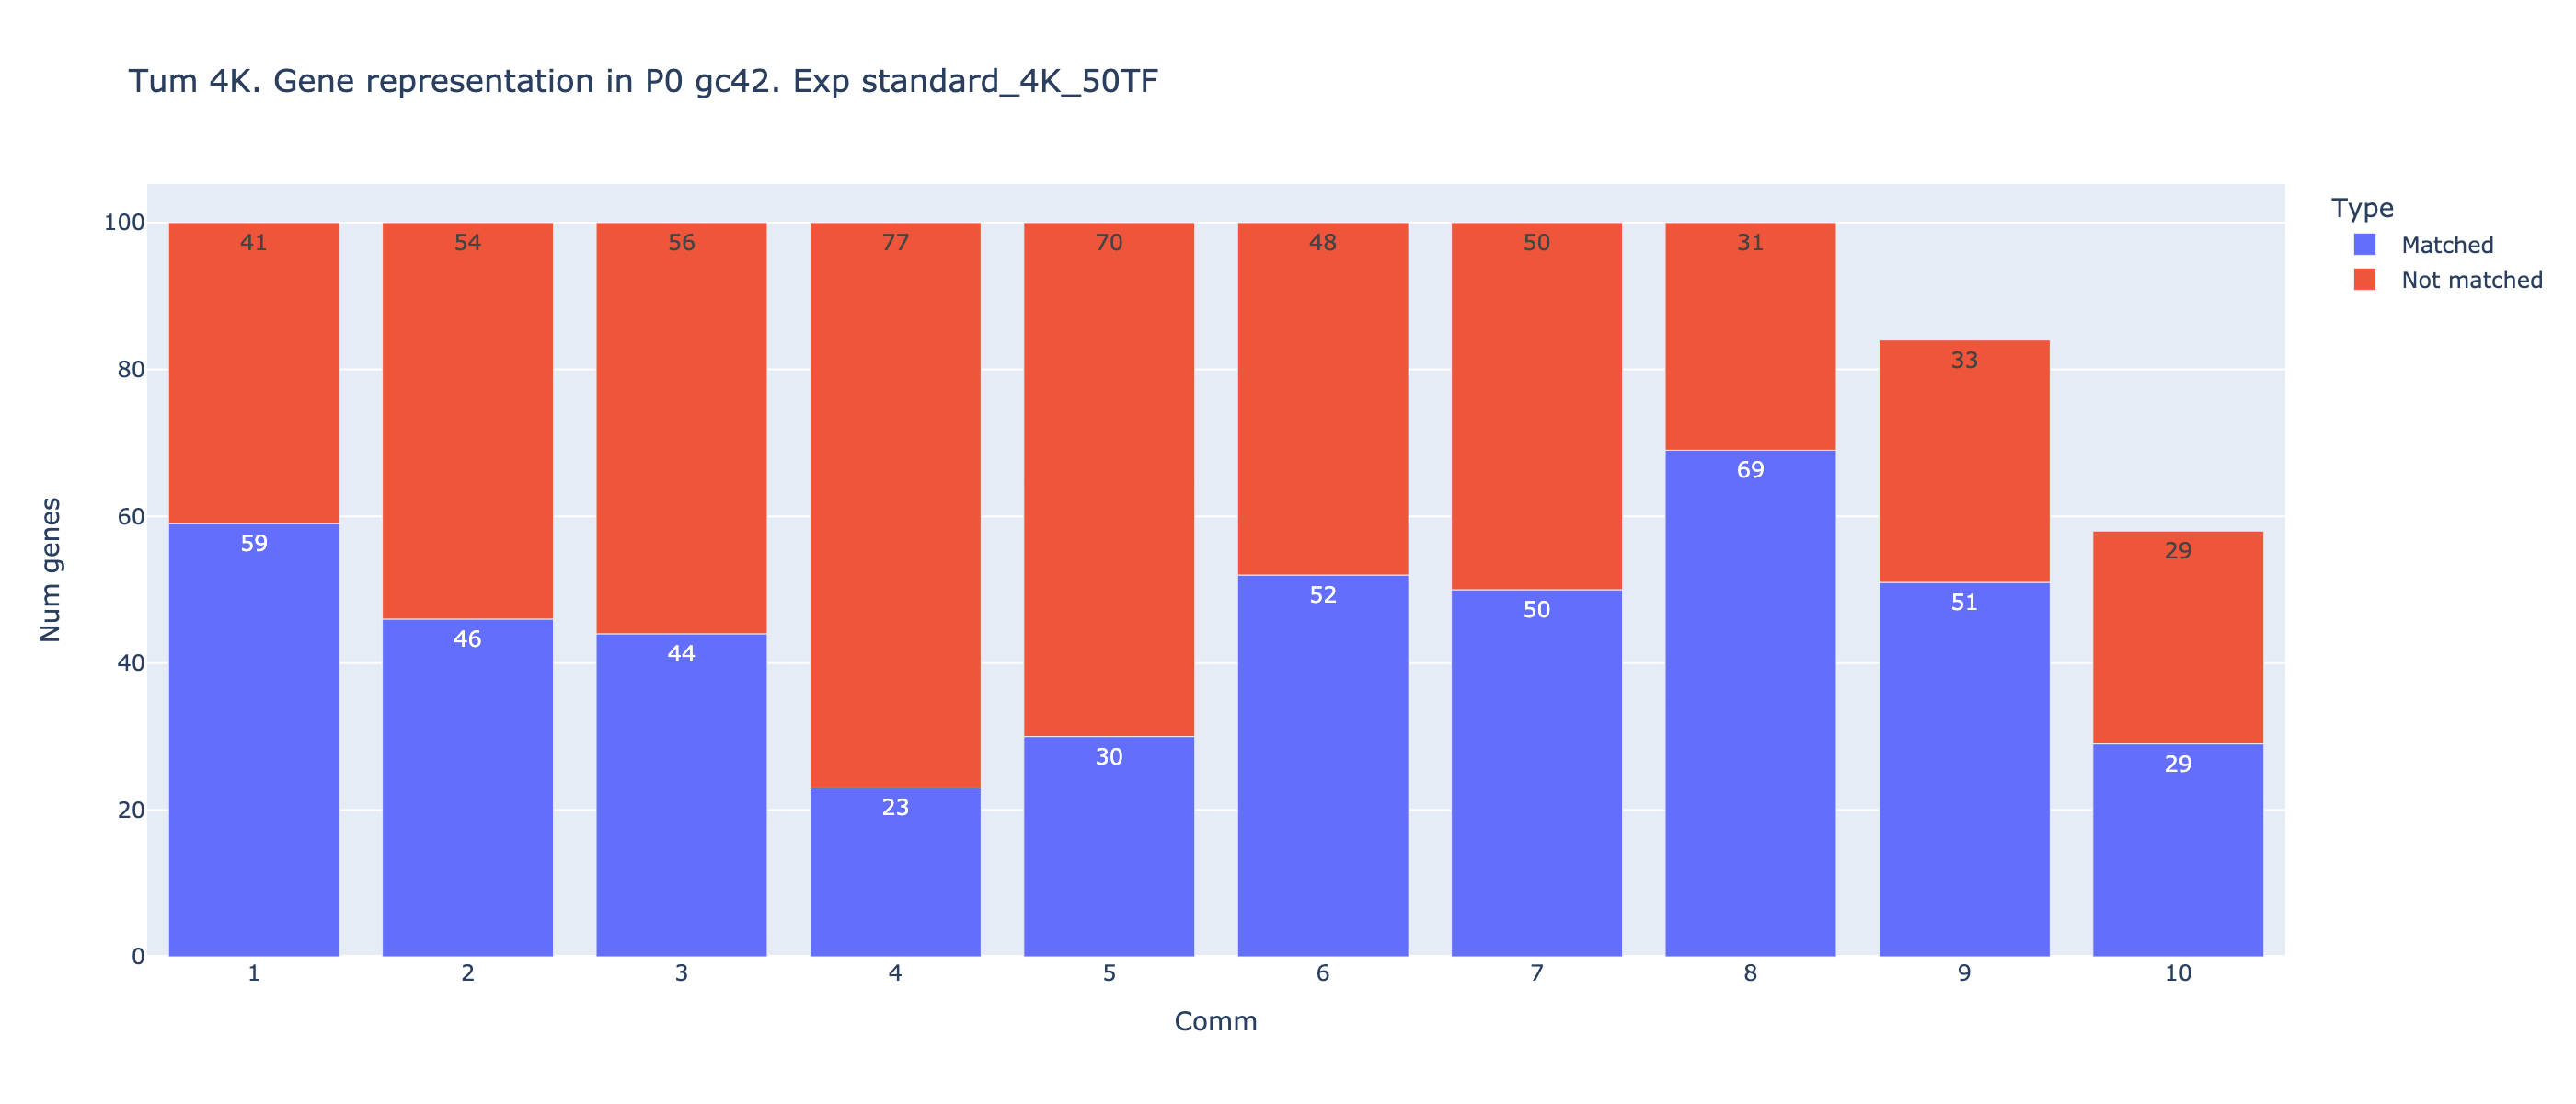
\includegraphics[width=\textwidth,keepaspectratio]{Sections/Network_I/Resources/P0/4K_p0_modConMev_rep_standard_4K_50TF.png}
        \caption{The most relative varied genes}
    \end{subfigure}
    \hfill
    \begin{subfigure}[b]{0.47\textwidth}
        \centering
        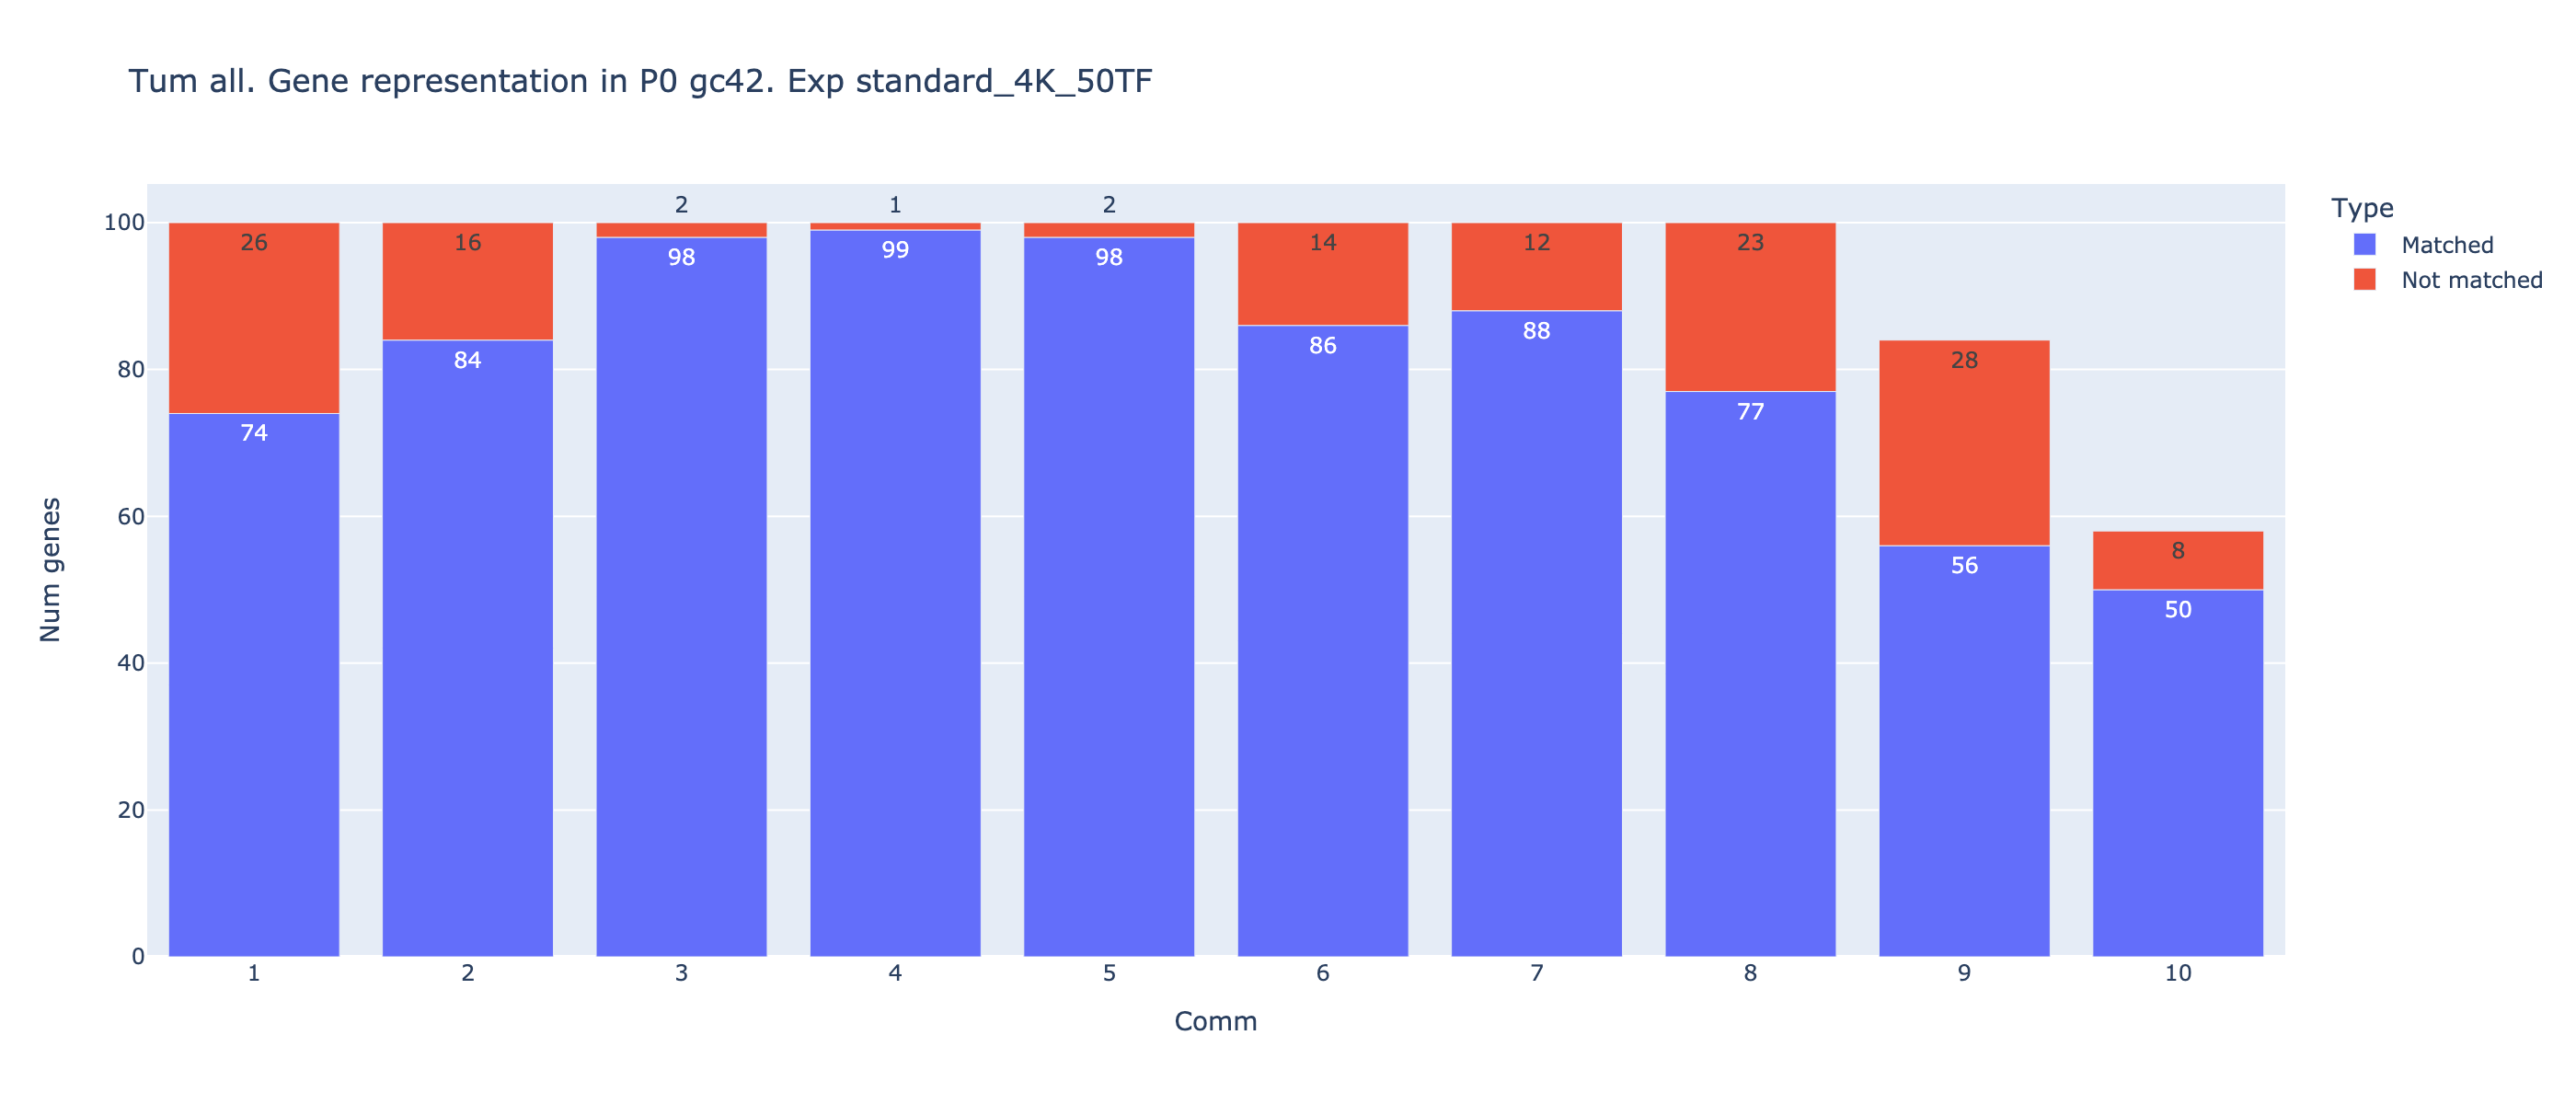
\includegraphics[width=\textwidth,keepaspectratio]{Sections/Network_I/Resources/P0/10K_p0_modConMev_rep_standard_4K_50TF.png}
        \caption{All the genes expressed}
    \end{subfigure}
    \hfill
    \caption{Genes found in the tumour dataset for each network community. The top 100 genes are selected by ModCon score. A) Is when the tumour dataset is restricted to the top most varied genes B) Includes all the expressed genes in the tumour dataset. }
    \label{fig:N_I:p0_mev_rep}
\end{figure}


\subsubsection{Conclusion}

So far in this section all of the experiments were performed with networks that have been minimum 50 connections per Transcription Factor gene. This value was pseudo-random chosen with the hope to prioritise the TFs in the network. Moreover, this was made on the assumption that the Leiden community detection algorithm is agnostic at the nodes' number of connection. Given the poor results in the MIBC subtyping this assumption came to scrutiny. 

Lowering the minimum number of edges per TF to 10 had a drastic improvements in the performance. There are more communities found and the modularity score across all three network increased. In addition, when computing all the expressed genes were considered instead of looking at just the most varied ones. The clustering and communities were re-analysed but similar trends were found. The weight modifiers change the networks, there are changes in communities but no significant difference in the MIBC subtypes. 

The following changes are considered in the next section 1) Analyse the effect of TFs in the networks to find the most suitable value 2) Use the entire healthy dataset to increase the gene representation in the tumour,  3) a different community detection was analysed.



\newpage


% Reason 2 - Scatter biological pathways 
Further on, when we look at the biology of each community we could see that there a lot shared pathways across communities. This include PDGF, CCKR, apoptosis and others. This gives the impression that the approach developed did the contrary from the intended behaviour, instead of isolating the biological processes it scattered through the network. The pathways were discovered through the Gene Ontology tool using PANTHER Pathway option and \textbf{no correction}; the latter because the majority of the genes inputted were \textbf{not} given significant results. This further strengthen our intuition that this approach is not providing the intended results.

Figures I need to support for the above argument:
\begin{itemize}
    \item Pick 2-3 pathways from the ones found and highlight in the network.
    \item Maybe put the Network with annotations?
\end{itemize}

% Reason 3 - Effect of the TF. but this really is 
While performing the biological interpretation, looking at the genes selected by ModCon score, it can be clearly noticed that the TF genes play a major role in the networks. The reason for this is that in this set of experiment we enable 50 edges for each Transcription Factor, thus biasing the network for these genes. Definitely, this parameter have a large impact of ModCon. Therfore, we performed an experiment with a lower number of edges per TF and we found out that there are more communities with fewer communties.
Figure supporting the above:
\begin{itemize}
    \item How many of the genes selected from the ModCon are a TF? Give some stats
    \item The sub-graph where only the ModCon genes are selected for each community; with the size of the TF \ref{fig:N_1:tf_comp}
\end{itemize}

